%%%%%%%%%%%%%%%%%%%%%%%%%%%%%%%%%%%%%%%%%%%%%%%%%%%%%%%%%%%%
% Author: Étienne André
% Modified by: Jacques Gangloff
% Date  : 2025/01
% Distributed with the hope that it will be useful
%%%%%%%%%%%%%%%%%%%%%%%%%%%%%%%%%%%%%%%%%%%%%%%%%%%%%%%%%%%%

%%%%%%%%%%%%%%%%%%%%%%%%%%%%%%%%%%%%%%%%%%%%%%%%%%%%%%%%%%%%
% UNCOMMENT THIS LIGNE FOR VERSION WITH COMMENTS
% \def \VersionWithComments{}
% UNCOMMENT THIS LIGNE FOR DRAFT VERSION
% \def \DraftVersion{}
%%%%%%%%%%%%%%%%%%%%%%%%%%%%%%%%%%%%%%%%%%%%%%%%%%%%%%%%%%%%

\ifdefined\VersionWithComments
	\def \DraftVersion{}
\fi

\documentclass[a4paper,12pt]{article}

%%%%%%%%%%%%%%%%%%%%%%%%%%%%%%%%%%%%%%%%%%%%%%%%%%%%%%%%%%%%
% GENERAL PACKAGES
%%%%%%%%%%%%%%%%%%%%%%%%%%%%%%%%%%%%%%%%%%%%%%%%%%%%%%%%%%%%

\usepackage[french]{babel}
\usepackage{geometry}
\geometry{a4paper, top=1cm, left=2cm, right=2cm, bottom=1cm, nohead, includefoot} % includehead


%%%%%%%%%%%%%%%%%%%%%%%%%%%%%%%%%%%%%%%%%%%%%%%%%%%%%%%%%%%%
% BEGIN Watermarking
%%%%%%%%%%%%%%%%%%%%%%%%%%%%%%%%%%%%%%%%%%%%%%%%%%%%%%%%%%%%
\ifdefined\DraftVersion
	\usepackage{draftwatermark}
	\SetWatermarkText{brouillon}
	\SetWatermarkScale{8}
	\SetWatermarkColor[gray]{0.85}
\fi
% END Watermarking
\usepackage[svgnames,dvipsnames,table]{xcolor}

%%%%%%%%%%%%%%%%%%%%%%%%%%%%%%%%%%%%%%%%%%%%%%%%%%%%%%%%%%%%
% BIBLIOGRAPHY
%%%%%%%%%%%%%%%%%%%%%%%%%%%%%%%%%%%%%%%%%%%%%%%%%%%%%%%%%%%%
\usepackage{csquotes}
\usepackage[maxbibnames=20,url=false,doi=false,sorting=ydnt]{biblatex}
\addbibresource{all.bib}

%%%%%%%%%%%%%%%%%%%%%%%%%%%%%%%%%%%%%%%%%%%%%%%%%%%%%%%%%%%%
% HYPERLINKS
%%%%%%%%%%%%%%%%%%%%%%%%%%%%%%%%%%%%%%%%%%%%%%%%%%%%%%%%%%%%
\usepackage{hyperref}
\hypersetup{
    colorlinks=true,
    linkcolor=blue,
    filecolor=magenta,      
    urlcolor=cyan,
    pdftitle={Rapport d'activité},
    pdfpagemode=FullScreen,
    }

%%%%%%%%%%%%%%%%%%%%%%%%%%%%%%%%%%%%%%%%%%%%%%%%%%%%%%%%%%%%
% FORMATTING ACCORDING TO THE TEMPLATE STYLE
%%%%%%%%%%%%%%%%%%%%%%%%%%%%%%%%%%%%%%%%%%%%%%%%%%%%%%%%%%%%
\usepackage{sectsty}
\usepackage{titlesec}
\usepackage{fontspec}
\usepackage[listings]{tcolorbox}
\tcbuselibrary{most}
\usepackage{blindtext}
\usepackage{booktabs}
\usepackage{wrapfig}
\usepackage{float}


\titleformat{\section}{\normalfont\large\bfseries\color{RoyalBlue}}{}{0em}{}
\renewcommand{\thesubsection}{\arabic{subsection}}
\titleformat{\subsection}{\normalfont\normalsize\color{orange}}{\thesubsection.}{1em}{}
\renewcommand{\thesubsubsection}{\arabic{subsubsection}}
\titleformat{\subsubsection}{\normalfont\small\color{RoyalBlue!50}}{\thesubsection.\thesubsubsection.}{0.5em}{}

\newcommand{\Separation}{\noindent{\color{black!40}\rule{\textwidth}{2pt}}}
\newcommand{\separation}{\noindent{\color{black!40}\rule{\textwidth}{1pt}}}

\newtcolorbox{flipbox}[2][]{
enhanced,colframe=RoyalBlue,colback=Apricot!15,fonttitle=\bfseries,
flip title={interior hidden},title={#2},#1}


%%%%%%%%%%%%%%%%%%%%%%%%%%%%%%%%%%%%%%%%%%%%%%%%%%%%%%%%%%%%
% COMMENTS
%%%%%%%%%%%%%%%%%%%%%%%%%%%%%%%%%%%%%%%%%%%%%%%%%%%%%%%%%%%%

\ifdefined \VersionWithComments
	\newcommand{\instructionsSection}[1]{{\color{blue}[\textbf{Instructions section 27}: #1]}}
\else
	\newcommand{\instructionsSection}[1]{}
\fi

\newcommand{\instructions}[1]{{\color{black}#1}}


\title{Avancement de grade 2025}
\author{Jacques Gangloff}

\sloppy

%%%%%%%%%%%%%%%%%%%%%%%%%%%%%%%%%%%%%%%%%%%%%%%%%%%%%%%%%%%%
%%%%%%%%%%%%%%%%%%%%%%%%%%%%%%%%%%%%%%%%%%%%%%%%%%%%%%%%%%%%
\begin{document}
%%%%%%%%%%%%%%%%%%%%%%%%%%%%%%%%%%%%%%%%%%%%%%%%%%%%%%%%%%%%
%%%%%%%%%%%%%%%%%%%%%%%%%%%%%%%%%%%%%%%%%%%%%%%%%%%%%%%%%%%%

% Use the pretty cool UnistraA font as default
\setmainfont{UnistraA}[ 
    Extension = .ttf,
    UprightFont = *-Regular,
    ItalicFont = *-Italic,
    BoldFont = *-Bold,
    BoldItalicFont = *-BoldItalic
]

\ifdefined\VersionWithComments

	\textcolor{red}{This is the version with comments.
	To disable comments, comment out line~6 in the \LaTeX{} source.}
	
	\medskip
	
\fi

{
	\Huge\bfseries\color{gray}
	\noindent{}Rapport d'activités\footnote{\url{https://github.com/jacqu/rapport_activite}}
}

\bigskip

\noindent\rule{\textwidth}{2pt}

\medskip

{\em
\def\arraystretch{2}
\noindent{}\begin{tabular}{l l @{\hspace{3em}} l l}
	Nom d'usage & \textbf{GANGLOFF} & Prénom : & \textbf{JACQUES} \\
	Corps : & \textbf{PROFESSEUR DES UNIVERSITES} & Grade : & \textbf{1E CL.} \\
	Discipline/section : & \textbf{ROBOTIQUE/61} \\
\end{tabular}
}

\medskip

\noindent\rule{\textwidth}{2pt}


%%%%%%%%%%%%%%%%%%%%%%%%%%%%%%%%%%%%%%%%%%%%%%%%%%%%%%%%%%%%
%%%%%%%%%%%%%%%%%%%%%%%%%%%%%%%%%%%%%%%%%%%%%%%%%%%%%%%%%%%%
\section{Synthèse du parcours professionnel et contexte d'exercice}
%%%%%%%%%%%%%%%%%%%%%%%%%%%%%%%%%%%%%%%%%%%%%%%%%%%%%%%%%%%%
%%%%%%%%%%%%%%%%%%%%%%%%%%%%%%%%%%%%%%%%%%%%%%%%%%%%%%%%%%%%

% Présentation chronologique des principales étapes de la carrière faisant apparaître les éléments les plus significatifs (diplômes, positions, principales responsabilités et activités) 
% Présentation de l’évolution éventuelle des activités 
% Présentation des formations suivies notamment concernant vos activités pédagogiques
% Présentation chronologique des principales étapes de la carrière faisant apparaître les éléments les plus significatifs (diplômes, positions, principales responsabilités et activités) (rubrique limitée à 6000 caractères, blancs non compris, soit 2 pages maximum)

Ce rapport se focalise plus particulièrement sur la période qui a suivi ma dernière promotion, à savoir de septembre 2012 jusqu'à février 2025. Cette section, qui présente le contexte global de ma trajectoire professionnelle, est la seule à couvrir l'ensemble de ma carrière.

\subsection{Curriculum Vitae}

\begin{table}[H]
    \centering
    \begin{tabular}{ll}
    \toprule
        1992	& Diplôme d'ingénieur de l'INSA Strasbourg\\
        1995	& Agrégation de génie électrique à l'ENS Cachan\\
        1996	& DEA << Photonique et Image >>\\
        1999	& Thèse de doctorat\\
        2000	& Maître de conférences à l’université Louis Pasteur de Strasbourg\\
        2004	& Habilitation à diriger les recherches\\
        2005	& Professeur des universités à l’université de Strasbourg\\
        2012    & Promotion 1E CL.\\
    \bottomrule
    \end{tabular}
    \caption{Curriculum vitae}
    \label{tab:CV}
\end{table}

Je suis titulaire de la prime individuelle, composante 3, du Régime Indemnitaire des
Personnels Enseignants-Chercheurs (RIPEC) depuis le 1er octobre 2024.

\subsection{Responsabilités actuelles}

\begin{itemize}
    \item Editeur associé du journal \textit{IEEE Robotics and Automation Letters} depuis 2024.
    \item Président du comité d’experts scientifiques de Télécom Physique Strasbourg depuis 2022.
    \item Coresponsable du master IRIV depuis 2015 (200 étudiants en moyenne).
    \item Membre élu du conseil de Telecom Physique Strasbourg depui 2010.
    \item Membre élu du conseil de perfectionnement de Telecom Physique Strasbourg depuis 2010.
    \item Responsable du parcours AR (Automatique et Robotique) du Master IRIV depuis 2005 (25 étudiants en moyenne).
\end{itemize}


\subsection{Responsabilités antérieures}

\begin{itemize}
    \item Responsable du département i2S (Ingénierie des Signaux et Systèmes) de Telecom Physique Strasbourg de 2017 à 2022 (50 étudiants en moyenne).
    \item Responsable adjoint de l'équipe AVR du laboratoire ICube de 2012 à 2017.
    \item Membre nommé du CNU 61 de 2011 à 2015.
    \item Membre du comité d’experts scientifiques 61/63 de l’université de Strasbourg de 2011 à 2022.
    \item Animateur de l'axe transverse <<Environnement et Développement Durable>> du laboratoire ICube de 2009 à 2013.
    \item Responsable du département TIC (Technologies de l'Information et de la Communication) de Telecom Physique Strasbourg de 2009 à 2017 (50 étudiants en moyenne).
    \item Responsable de l'option ISAV (Ingénierie des Systèmes, Automatique et Vision) de Telecom Physique Strasbourg de 2004 à 2014 (15 étudiants en moyenne).
\end{itemize}

\subsection{Activités scientifiques}

Depuis 2012, j'ai effectué deux changements thématiques : 2012 marque le début de mes activités en robotique parallèle à câbles après une période de 2003 à 2012 consacrée à la robotique médicale avec un focus particulier sur la chirurgie cardiaque robotisée à cœur battant. Ce premier changement assez radical de thématique fut notamment motivé par le sentiment d'avoir exploré de façon suffisamment exhaustive les TRL bas de ce champ applicatif. Nos travaux sur des preuves de concept avaient notamment été distingués à l'époque par le prix du meilleur article de la revue \textit{IEEE transactions on Robotics and Automation}. 

Le chemin restant à parcourir concernait essentiellement des briques de pré-maturation dont le financement était à l'époque assez difficile à justifier étant donné le contexte très fermé du paysage de la propriété intellectuelle dans ce domaine. En clair, la plupart des brevets dans ce domaine étaient détenus par une seule entreprise qui était devenue incontournable.

Outre ce sentiment d'avoir fait le tour de la question, c'est aussi une volonté de m'investir plus directement dans des technologies pour l'environnement qui m'a poussée à m'intéresser aux robots parallèles à câbles. En effet, leur espace de travail très grand est l'un des rares qui soit compatible avec des applications extérieures, comme la surveillance d'écosystèmes ou l'agriculture raisonnée. Enfin, le côté frugal de ce type d'architecture a aussi compté dans mon choix, ce type de robot ayant un ratio volume de travail sur masse du robot imbattable, si l'on exclut les robots aériens.

Et c'est justement cette caractéristique partagée avec les robots aériens qui m'a poussée à opérer mon dernier changement thématique vers la robotique aérienne en 2018. Cette transition fut beaucoup plus douce que la première dans la mesure où nous nous sommes intéressés à la manipulation aérienne suspendue qui peut être considérée comme un cas particulier de robot à câble. Là aussi, c'est la frugalité du système en termes de complexité mécanique, de consommation de matières premières et d'énergie qui a dicté cette transition.

Je suis sur le point d'opérer un nouveau changement thématique relativement naturel de la manipulation aérienne vers la robotique frugale. Je participe actuellement aux travaux du PEPR << Accélération Robotique >> et je contribue plus particulièrement aux réflexions du projet << Robotique frugale pour la transition >> qui est dans la continuité de mes choix scientifiques depuis 2012.

%------------------------------------------------------------
\Separation{}
%------------------------------------------------------------


%%%%%%%%%%%%%%%%%%%%%%%%%%%%%%%%%%%%%%%%%%%%%%%%%%%%%%%%%%%%
%%%%%%%%%%%%%%%%%%%%%%%%%%%%%%%%%%%%%%%%%%%%%%%%%%%%%%%%%%%%
\section{Investissement pédagogique}
%%%%%%%%%%%%%%%%%%%%%%%%%%%%%%%%%%%%%%%%%%%%%%%%%%%%%%%%%%%%
%%%%%%%%%%%%%%%%%%%%%%%%%%%%%%%%%%%%%%%%%%%%%%%%%%%%%%%%%%%%

%%%%%%%%%%%%%%%%%%%%%%%%%%%%%%%%%%%%%%%%%%%%%%%%%%%%%%%%%%%%
\subsection{Présentation synthétique de l'activité d'enseignement}
%%%%%%%%%%%%%%%%%%%%%%%%%%%%%%%%%%%%%%%%%%%%%%%%%%%%%%%%%%%%

% Présentation de l’activité d’enseignement : principaux enseignements en mettant l’accent sur les thématiques enseignées, les pratiques pédagogiques, les responsabilités pédagogiques particulières : création d’un enseignement, d’une formation, direction d’une équipe pédagogique…  (la rubrique 1 est limitée à 6000 caractères, blancs non compris, soit environ 2 pages)

J’enseigne en deuxième et troisième année de formation d’ingénieur sous statut
étudiant de l’école « Télécom Physique Strasbourg ». La plupart de mes
enseignements sont mutualisés avec le master IRIV et les cohortes comprennent donc aussi des étudiants inscrits en M1 ou en M2. Un nombre significatif de ces étudiants est élève ingénieur de l’INSA Strasbourg, inscrit en double diplôme au master IRIV. J’interviens en cours, en travaux pratiques et en projet.

Tous mes cours sont basés sur des supports de type PowerPoint projetés par vidéoprojecteur. En moyenne, je projette 20 diapositives par heure de cours. Mes cours contiennent des séquences d’exercices intégrés et des démonstrations en direct sur des logiciels comme Matlab/Simulink. À la fin de tous les chapitres, je propose aux étudiants un QCM de 5 à 15 minutes qui permet de tester l’assimilation des connaissances [\href{https://docs.google.com/forms/d/18JizlS3drjelkc4IQsd0PguedCdYTxuA80YoaMUxwCc}{exemple de QCM}]. Ce QCM est corrigé et commenté en cours juste après. Cette séquence me permet d’améliorer l’interaction avec mes
étudiants. Elle est l’occasion pour moi de déceler rapidement des problèmes de compréhension et pour eux, de vérifier leur niveau par rapport à l’ensemble du groupe (des statistiques anonymes sont données lors du débriefing).

En 2023, j’ai créé un nouveau cours de drone (15HTD) qui comprend un TP de deux heures utilisant des quadricoptères destinés à l’éducation. Ce TP me sert aussi de démonstrateur de nos activités d'enseignement lors des journées portes ouvertes organisées tous les ans par l'école. J’ai aussi organisé l’insertion au sein de cet enseignement d’un complément de 4 heures assuré par un intervenant extérieur issu du monde socio-économique. J’ai remis à jour et étendu mon cours de robotique (32HTD) en 2022. En 2021, j’ai complètement modifié mon cours d’ingénierie durable (34HTD) de manière à y introduire plus d’études de cas. Enfin, j’ai monté un cours d’initiation à la recherche (8HTD) en 2020 qui est dispensé à l’ensemble du M2 IRIV.

En 2019, j'ai développé un programme de quizz capable de vérifier automatiquement la réponse donnée sous une forme mathématique symbolique. J'utilise pour cela le moteur symbolique de la calculatrice TI NSpire, et grâce à ses capacités de simplification, le programme est capable de détecter une réponse juste ou fausse, quelle que soit la forme de la réponse saisie (factorisée ou non, simplifiée ou non). J'ai organisé l'achat de 70 calculatrices de ce type financées par l'école, notamment pour le cours de robotique dont les problèmes sont très calculatoires. J'ai utilisé ce QCM en cours et en examen. L'avantage en examen, c'est que l'étudiant peut savoir si sa réponse est juste ou fausse (sans dévoiler le résultat) avant de passer à la question suivante. Sachant que les problèmes de robotique sont souvent très incrémentaux, ça lui permet de valider chaque étape du problème avec certitude avant de passer à la question suivante. Ce programme écrit en langage Lua est disponible sur GitHub\footnote{\url{https://github.com/jacqu/LuaQ}} et une vidéo tutorielle est disponible sur YouTube\footnote{\url{https://youtu.be/S9-Bd0KnUwM}}.

En 2017, j'ai monté 3 séances de travaux pratiques de 4 heures chacune, basées sur des Lego Mindstorms et la boîte à outils Simulink <<RPIt>>\footnote{\url{https://github.com/jacqu/rpit}} que j'ai développée dans le cadre de mes recherches. Ces nouvelles maquettes low-cost (300 € par maquette, 4 maquettes par TP, 12 maquettes en tout) visaient à remplacer du matériel vieillissant et onéreux (6000 € par maquette de la société Quanser Consulting) qui n'avait pas donné satisfaction en termes de robustesse ni de performance pédagogique. Ces nouvelles maquettes sont en fonctionnement depuis maintenant 8 ans et donnent entière satisfaction. J'ai été invité en 2024 à faire une présentation devant mes collègues du GdR robotique sur les retours d'expérience en matière de démarche frugale pour l'enseignement à Télécom Physique Strasbourg. J'ai ainsi pu partager quelques statistiques concernant ces trois travaux pratiques sur cette période de 8 ans (évaluation des étudiants, fiabilité du matériel, coût, partage des ressources pédagogiques). Ce point sera détaillé dans la section <<Diffusion, rayonnement>> ci-dessous.

%%%%%%%%%%%%%%%%%%%%%%%%%%%%%%%%%%%%%%%%%%%%%%%%%%%%%%%%%%%%
\subsection{Présentation des enseignements}
%%%%%%%%%%%%%%%%%%%%%%%%%%%%%%%%%%%%%%%%%%%%%%%%%%%%%%%%%%%%

% Présentation synthétique des enseignements (par exemple sous forme de tableau) faisant apparaitre le niveau (L.M.D), le type de formation (formation initiale/continue, professionnelle, présentielle/à distance) la nature (cours, TD, TP, encadrement de travaux de fin d’étude et de stages), les effectifs, le volume.  

Voici la liste des enseignements que j'ai dispensés durant les 5 dernières années :
\begin{itemize}
    \item Drones: Design, Build and Control (CM+TP, ING3/M2)
    \item Robotique : manipulation et commande (CM+TP, ING3/M2)
    \item Vision et commande (CM+TP, ING3/M2)
    \item Asservissements visuels rapides (CM+TP, ING3/M2)
    \item Technologie des asservissements (CM, ING3/M2)
    \item Temps-réel et systèmes embarqués (CM+TP, ING3/M2)
    \item Commande prédictive (CM, ING3/M2)
    \item Projets tutorés (Projet, ING3)
    \item Initiation à la recherche (CM, M2)
    \item Commande numérique (CM+TP, ING2/M1)
    \item Robotique et automatismes (CM+TP, ING2/M1)
    \item Ingénierie durable (CM+Projet, ING2/M1)
\end{itemize}
{\small

ING3 : dernière année du cycle de formation ingénieur

ING2 : deuxième année du cycle de formation ingénieur
}

Le détail de tous mes enseignements depuis ma dernière promotion est donné dans l'annexe \ref{sec:annexe_enseignements}. Sur la période 2012--2025, mon \textbf{service annuel moyen s'élève à 240 heures} équivalent TD. J'ai effectué en moyenne 48 heures supplémentaires par an. J'ai été gratifié en moyenne de 53 heures par an pour des responsabilités et missions diverses. 


%%%%%%%%%%%%%%%%%%%%%%%%%%%%%%%%%%%%%%%%%%%%%%%%%%%%%%%%%%%%
\subsection{Responsabilités pédagogiques}
%%%%%%%%%%%%%%%%%%%%%%%%%%%%%%%%%%%%%%%%%%%%%%%%%%%%%%%%%%%%

% Responsabilités pédagogiques, en particulier direction, animation, montage de formations, notamment à l’international, fabrication et utilisation de ressources pédagogiques, soutien à l’orientation, soutien à la promotion sociale et à l'insertion professionnelle, soutien à l'entrepreneuriat, etc. 

\subsubsection{Coresponsabilité du master IRIV}

Depuis 2015, j’assume avec mon collègue Christian Heinrich la coresponsabilité du master IRIV. Ce master est l’un des plus gros de l’université de Strasbourg, avec plus de 200 étudiants en M1 et M2. Avec mon collègue, nous nous partageons équitablement les tâches administratives de gestion de ce master et nous prenons toutes les décisions de façon collégiale. Voici les chantiers liés à cette responsabilité dans lesquels je me suis particulièrement impliqué :
\begin{itemize}
    \item 2015 : Première refonte du site web (MediaWiki)
    \item 2016 : Evaluation HCERES
    \item 2016 : Refonte des maquettes pédagogiques du master
    \item 2017 : Elaboration de l'offre de formation 2018-2022 avec notamment la création d'un nouveau parcours <<Topographie et Photogrammétrie>> en partenariat avec l'INSA
    \item 2017 : Négotioation de la convention de coaccréditation avec l'INSA
    \item 2018 : Deuxième refonte du site web\footnote{\url{https://www.master-iriv.fr}} (Google sites)
    \item 2019 : Ouverture du M2 aux étudiants étrangers << Incoming >> de l’INSA Strasbourg via un avenant à la convention de coaccréditation
    \item 2022 : Evaluation HCERES
    \item 2022 : Transition du recrutement de eCandidat vers la plateforme MonMaster
    \item 2022 : Transition du recrutement des étudiants extracommunautaires de eCandidat vers la plateforme EtudesEnFrance
    \item 2023 : Démarche compétence (référentiel de compétences, matrices croisées, fiche RNCP)
    \item 2023 : Elaboration de la nouvelle offre de formation 2024—2028
    \item 2023 : Introduction d’un examen en ligne pour le recrutement en M1
    \item 2024 : Renégociation de l’accord de coaccréditation avec l’INSA Strasbourg
\end{itemize}

Voici les principales tâches récurrentes de gestion du master dans lesquelles je suis particulièrement impliqué :
\begin{itemize}
    \item Réunions d’information à destination de tous les publics concernés
    \item Relations avec l'INSA Strasbourg
    \item Participation aux réunions du bureau de direction de Télécom Physique Strasbourg (réunion mensuelle de 2 heures 30)
    \item Animation des jurys de semestre et de diplôme (7 réunions dans l’année)
    \item Commission pédagogique de filtrage des admissions sur titre (environ 180 dossiers à analyser par an)
    \item Animation du conseil de perfectionnement (2 réunions dans l’année)
    \item Présentation des points soumis au vote liés au master au conseil d'école
    \item Mise à jour des maquettes pédagogiques et des modalités d'enseignement et de contrôle des connaissances
    \item Mise à jour du site web
    \item Cérémonie de remise des diplômes (discours, remise des diplomes)
\end{itemize}

Ce master est en forte croissance. Depuis notre prise de fonction, les effectifs sont passés de 150 à 210 étudiants.

\subsubsection{Responsabilité de département}

J’ai assumé depuis 2009 jusqu’en septembre 2022 la responsabilité d'un département de l'école d'ingénieurs (dénommé département <<TIC>> de 2009 à 2017 et département <<i2S>> depuis 2017). Ce département comptait en moyenne 50 étudiants qui se répartissaient en dernière année dans trois options. J’ai notamment eu à gérer le chantier de la structuration de ce département (auparavant, l'école n'était pas organisée en départements), de l’intégration de l’option électronique à ce département, ainsi que la réorganisation de l’offre des cours optionnels. J'animais les discussions sur les évolutions de la maquette pédagogique, j'assurais de manière récurrente la communication à destination des étudiants des informations concernant ce département, je pilotais la procédure de choix de cours optionnels et d’options de troisième année et je gérais l’interface entre la direction de l’école et les responsables d’options. J’ai transmis cette responsabilité à ma collègue Iuliana Bara afin de pouvoir me concentrer sur deux nouveaux projets ANR qui ont débuté en 2022.

\subsubsection{Responsabilité de parcours de master}

Depuis 2005, je suis responsable du parcours <<Automatique et Robotique>> (AR) du master IRIV. C’est le parcours de M2 dont l’effectif est le plus élevé (25 étudiants en moyenne) notamment en raison d’un effectif d’étudiants de l’INSA Strasbourg en forte croissance ces dernières années. Je me suis occupé des relations avec l’INSA depuis ma prise de fonction. Les relations entre le master et l'INSA se sont encore rapprochées avec ma prise de fonction en 2015 à la tête du master. La convention de coaccréditation signée en 2015 a par exemple entériné les relations étroites qui ont été tissées de façon informelle durant les dix années qui ont précédé. Je gère la communication avec les référents de l’INSA et sa direction des études. Au fil des années, nous avons optimisé la maquette pédagogique du parcours AR de manière à ce qu’elle s’articule parfaitement avec celle de la cinquième année des différentes spécialités de l’INSA. Avec l'ouverture à la spécialité <<plasturgie>> en 2019, ce sont maintenant 4 spécialités de l'INSA qui sont compatibles avec le parcours. Ces optimisations ont porté leurs fruits, car nous sommes actuellement le master de l’université qui accueille le plus d’étudiants de l’INSA Strasbourg en double diplôme. Les effectifs INSA sont passés d'une moyenne de 5 étudiants en 2012 à une moyenne de 15 ces 5 dernières années.

J’ai aussi développé le recrutement en provenance des pays de la francophonie via un MOOC dont l’épreuve de certification me sert de présélection à l’admission sur titre au parcours AR (ce MOOC est détaillé dans la section \ref{sec:ens_diffusion_rayonnement} ci-dessous).

Le gros du travail récurrent lié à cette fonction consiste à gérer les jurys de stage. Je préside notamment tous les jurys de soutenance des stages de tous les étudiants du parcours (3 journées complètes de soutenances dans l’année). La mission consiste aussi à animer des réunions d'information à destination des futurs candidats (notamment à l'INSA), à valider les conventions de stage de master ou encore à gérer les admissions sur titre.

\subsubsection{Responsabilité d'une option de dernière année de cycle ingénieur}

J'ai été responsable de l'option de troisième année <<ISAV>> de Télécom Physique Strasbourg jusqu'en 2014. Cette option comptait en moyenne 18 étudiants. J'étais chargé d'organiser les emplois du temps, d'animer les discussions pédagogiques avec les collègues enseignants, de présider les jurys de soutenance de fin d'études, de gérer les stages de fin d'études et de gérer la communication liée à l'option.

%%%%%%%%%%%%%%%%%%%%%%%%%%%%%%%%%%%%%%%%%%%%%%%%%%%%%%%%%%%%
\subsection{Diffusion, rayonnement, activités internationales.}
%%%%%%%%%%%%%%%%%%%%%%%%%%%%%%%%%%%%%%%%%%%%%%%%%%%%%%%%%%%%
\label{sec:ens_diffusion_rayonnement}

% Diffusion de la culture (humaniste) à travers le développement des sciences humaines et sociales et/ou de la culture scientifique, technique et industrielle, participation à des expositions, etc.
% Rayonnement et activités internationales dont la participation à la construction de l’espace européen de l’enseignement supérieur et de la recherche, la coopération internationale, etc. 

En novembre 2024, j'ai été invité à faire une présentation plénière aux journées du GdR robotique dans le cadre de son action prioritaire << Robotique et éducation >> qui s'intitulait : << Transition écologique et enseignement : bilan sur 15 ans à Télécom Physique Strasbourg >>. En effet, nous avons été précurseurs à Strasbourg en montant en 2009 un cours dont la thématique pourrait être qualifiée aujourd'hui de << DDRS >> pour Développement Durable et Responsabilité Sociétale (cf mon cours d'ingénierie durable). J'ai donc fait une présentation qui présente un bilan sur 15 ans de cet enseignement avec ses nouvelles problématiques émergentes liées aux critiques du technosolutionnisme. J'ai publié \href{https://youtu.be/gVKNGADG_mw}{une vidéo} sur YouTube se focalisant sur cette partie de ma présentation au GdR qui a eu un écho très favorable auprès de mes collègues roboticiens. L'autre partie a porté sur un bilan de l'application de principes de frugalité dans le montage de maquettes de travaux pratiques de robotique et de mécatronique depuis une dizaine d'années à Télécom Physique Strasbourg, avec mise à disposition de toutes les ressources pour les collègues intéressés. La présentation complète est disponible \href{https://www.gdr-robotique.org/rapports/?id=c93716b1cd6309bde1a84101b5ea847d}{sur le site du GdR Robotique}.

Suite à cette présentation, des collègues de l'INSA Strasbourg m'ont demandé de faire une conférence sur ces thématiques (transition écologique et technosolutionisme, robotique frugale) à destination de leurs étudiants ingénieurs dans le cadre de leur sensibilisation au DDRS.

\begin{wrapfigure}{R}{0.6\textwidth}
\centering
\vskip-4mm
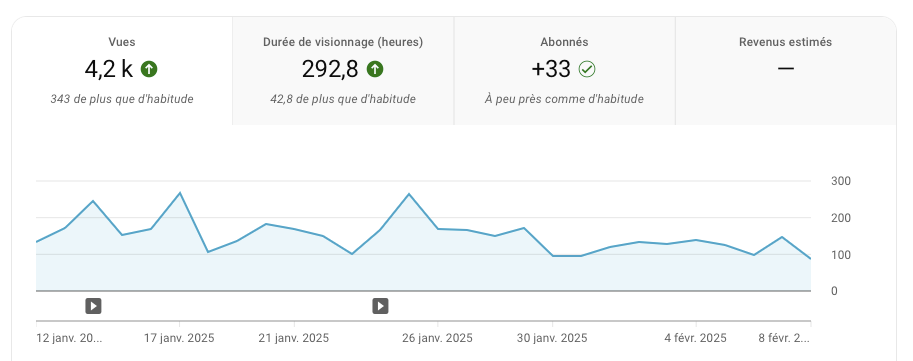
\includegraphics[width=0.6\textwidth]{YouTube.png}
{\em Statistiques YouTube récentes sur 28 jours}\vskip-4mm
\end{wrapfigure}
Tous mes cours sont enregistrés et disponibles sur YouTube\footnote{\url{https://www.youtube.com/@JacquesGangloff}}. Les statistiques de visionnage, les commentaires informels des étudiants et les évaluations des enseignements montrent que cette ressource leur est utile. Ma chaîne YouTube est dédiée essentiellement à l’enseignement. Elle compte à ce jour {\bf 9\;600} abonnés et totalise {\bf 62\;000} heures de visionnage. Même si l'essentiel du trafic provient de France métropolitaine (environ 30\% de la durée de visionnage totale), une bonne partie du trafic restant provient de la francophonie (Algérie, Maroc, Tunisie, Cameroun, Canada, Belgique).

Ma chaîne est associée à un MOOC hébergé par un site web\footnote{\url{https://www.rbotx.org}} que j’administre et qui permet d’accéder via un portail unique à toutes les ressources de mes cours (vidéos, fichiers des diapositives, compléments d’explications, fichiers des logiciels utilisés en cours, archives corrigées des examens, fichiers des travaux pratiques). Depuis 2018, date de création de ce MOOC, j'organise tous les ans des épreuves écrites et orales dans le cadre de ce MOOC : une épreuve d'admissibilité qui consiste à traiter un problème de robotique pendant 3 heures et une épreuve orale individuelle d'admissibilité qui consiste en une séquence de questions/réponses qui balaie tout le contenu du programme. Toutes les activités ayant trait à ce MOOC, y compris l’organisation des sessions d’examen, sont entièrement bénévoles.

\begin{flipbox}{Statistiques du MOOC $\rho$BOTx}   
   Depuis 2018, 337 candidats se sont inscrits à l'épreuve d'admissibilité,  21 ont validé l'épreuve d'admissibilité et ont été auditionnés individuellement lors d'une épreuve orale d'une heure, 8 ont validé les deux épreuves. Les 8 candidats ayant validé les deux épreuves se sont vus proposer un accès facilité au parcours <<Automatique et Robotique>> du master IRIV dont je suis responsable. Parmi eux, 5 ont intégré le master IRIV et l'un d'entre eux en est sorti major de promotion. Suite à cette belle performance, il a pu intégrer notre école d'ingénieur dont il est aussi sorti major. Il est actuellement en thèse à l'INRIA Rennes. J'ai récemment publié une vidéo sur le devenir des premiers lauréats du MOOC : \url{https://youtu.be/oJdGEGs9mM0}
\end{flipbox}

En 2017, j'ai publié un \href{https://amzn.eu/d/bexz1iP}{livre d'exercices de robotique} en auto-édition via Kindle Direct Publishing. C'est une compilation de 15 années de mes sujets d'examen de robotique avec une correction détaillée. Des QR codes sont disséminés un peu partout dans le livre : ils renvoient aux séquences exactes de mes vidéos YouTube où sont expliqués les concepts utiles à la section du livre où ils sont insérés. Mes étudiants ont une dizaine d'exemplaires à disposition à la bibliothèque de l'école afin de les aider dans leurs révisions. J'ai ajusté le prix de vente au minimum, que ce soit pour la version Kindle ou pour la version papier, de manière à rendre ce document le plus accessible possible. Par exemple, la version Kindle est actuellement au prix de {\bf 5 €}. Ce livre s'est écoulé à environ {\bf 300} exemplaires depuis sa sortie et bénéficie de bonnes évaluations sur Amazon ({\bf 4.3 sur 5} avec 11 évaluations).

%------------------------------------------------------------
\Separation{}
%------------------------------------------------------------


%%%%%%%%%%%%%%%%%%%%%%%%%%%%%%%%%%%%%%%%%%%%%%%%%%%%%%%%%%%%
%%%%%%%%%%%%%%%%%%%%%%%%%%%%%%%%%%%%%%%%%%%%%%%%%%%%%%%%%%%%
\section{Activité scientifique}
%%%%%%%%%%%%%%%%%%%%%%%%%%%%%%%%%%%%%%%%%%%%%%%%%%%%%%%%%%%%
%%%%%%%%%%%%%%%%%%%%%%%%%%%%%%%%%%%%%%%%%%%%%%%%%%%%%%%%%%%%
\newrefsection

%%%%%%%%%%%%%%%%%%%%%%%%%%%%%%%%%%%%%%%%%%%%%%%%%%%%%%%%%%%%
\subsection{Présentation synthétique des thématiques de recherche}
%%%%%%%%%%%%%%%%%%%%%%%%%%%%%%%%%%%%%%%%%%%%%%%%%%%%%%%%%%%%

% Présentation synthétique des thématiques de recherche : grands axes de recherches et apport dans le ou les domaines concernés (la rubrique 1 est limitée à 6000 caractères, blancs non compris, soit environ 2 pages) :

Dans mes choix scientifiques, j’ai toujours privilégié la prise de risque à la sécurité, la qualité à la quantité. Au bout de six à huit années de recherche, la thématique étudiée atteint souvent un stade de maturité qui nécessite d'aller trouver un nouveau souffle. J'avoue avoir complètement sous-estimé la difficulté de mon premier changement thématique vers la robotique parallèle à câbles. En effet, il s’agissait de rapidement monter en compétences et en crédibilité dans une discipline ayant déjà une longue antériorité en partant pratiquement de zéro et avec des financements très limités. 

Pourtant, ce virage, même s’il était serré, n’était pas à 90 degrés. En effet, certains concepts développés dans le cadre de la chirurgie cardiaque à cœur battant ont pu être exploités en robotique parallèle à câbles, comme l’utilisation d’actionneurs embarqués pour compenser une perturbation périodique. 

Il en a toutefois résulté une baisse significative de ma production scientifique durant la période 2014 -- 2019 que j’avais imaginée plus courte (aucune publication dans un journal et seulement 4 publications dans de bonnes conférences). Néanmoins, les articles \cite{2-BCLG19}, \cite{2-CWG20} et \cite{2-CAYD23} dans les revues \textit{IEEE Transactions on Robotics, Journal of Mechanisms and Robotics} et \textit{Mechanism and Machine Theory} ont récompensé ces années d'efforts par une reconnaissance de nos contributions au plus haut niveau. Ces contributions ont principalement porté sur l'amélioration des performances dynamiques de ce type de robot grâce à un asservissement visuel rapide exploitant une commande prédictive non linéaire. Nous avons ainsi pu montrer que l'ajout d'actionneurs embarqués et/ou la prise en compte de la flexibilité des câbles dans le modèle dynamique permettaient de remédier aux principaux inconvénients de ce type de robot : une flexibilité importante et une répétabilité limitée. Le projet ANR << DexterWide >> (2015 -- 2019), porté par Marc Gouttefarde du LIRMM et dont j'étais responsable scientifique pour ICube, nous a permis de gagner en compétences, notamment en bénéficiant de la grande et longue expertise du LIRMM dans ce domaine.

Le projet ANR jeune chercheur << eVISER >> (2018 -- 2021), porté par Sylvain Durand et auquel j'ai participé, nous a permis de financer la transition vers la manipulation aérienne. Cette transition s'est faite naturellement, dans la mesure où l'un des types d'actionneurs que nous avons embarqués dans un robot parallèle à câbles afin d'en améliorer la dynamique est un propulseur de drone. C'est la thèse d'Arda Yigit (voir annexe \ref{sec:theses}), financée par eVISER, qui a permis de faire décoller cette thématique au sein de l'équipe. Nos contributions portant sur la suspension élastique d'une plateforme aérienne omnidirectionnelle de manière à minimiser l'énergie consommée tout en maximisant les performances dynamiques et la précision, nous ont permis de gagner très rapidement une visibilité internationale dans une communauté scientifique vaste et bien établie. Les travaux d'Arda ont notamment débouché sur un article dans \textit{IEEE Robotics and Automation Letters} (RAL) \cite{2-YACD21} en 2021 et dans \textit{IEEE Transactions on Robotics} (TRO) \cite{2-YCAD23} en 2023.

Le projet ANR << STRAD >> (STReet Art Drone, 2022 -- 2026) que je coordonne porte sur une application très originale de la manipulation aérienne à la frontière entre technologie et art. Le but est de réaliser une fresque de très grande dimension avec un manipulateur aérien. Nous avons inclus dans le consortium une association qui organise le plus grand festival européen de street art à Grenoble, c'est notre lien avec le monde artistique. Le Gipsa-lab est aussi partenaire et apporte sa longue expérience dans les drones. Ce projet finance la thèse d'Ethan Niddam (voir annexe \ref{sec:theses}) dont les premiers résultats ont déjà permis la publication d'un article dans le journal \textit{IEEE Robotics and Automation Letters} \cite{2-NDCD24}. Par ailleurs, sa contribution à la thèse de Miguel Arpa Perozo, elle aussi dans le cadre de STRAD, lui a permis de cosigner un deuxième article dans cette même revue \cite{2-ANCDxx}.

Actuellement je concentre tous mes efforts dans la recherche de financements pour ma future thématique de recherche en robotique frugale. J'ai ainsi coordonné la soumission cette année d'un projet ANR dont la thématique centrale est la frugalité et qui exploite un actionnement aérien, donc pas tout à fait orthogonal avec ce que je fais actuellement. Ce projet a été déposé avec le LS2N et l'INRIA Rennes. Il inclut aussi des membres de mon équipe qui travaillent habituellement en robotique médicale, ce qui constitue une passerelle intéressante entre les différents thèmes de cette très grosse équipe. Je participe aussi activement aux travaux du PEPR << Accélération Robotique >> et, en particulier, je fais partie de l'équipe resserrée autour de Sébastien Briot qui rédige le projet << Robotique frugale pour la transition >>.

En conclusion, et a posteriori, je ne regrette absolument pas de m’être engagé dans cette voie scientifique aventureuse et changeante, car elle nous a permis, avec les collègues qui m'ont accompagné, de faire des contributions originales de premier plan et nous a amenés vers de nouvelles thématiques toujours plus prometteuses et extrêmement motivantes.


%%%%%%%%%%%%%%%%%%%%%%%%%%%%%%%%%%%%%%%%%%%%%%%%%%%%%%%%%%%%
\subsection{Publications et productions scientifiques }
%%%%%%%%%%%%%%%%%%%%%%%%%%%%%%%%%%%%%%%%%%%%%%%%%%%%%%%%%%%%

% Publications : présentation, en quelques lignes, des 5 publications (ou brevets, logiciels, compte rendus, rapports) jugées les plus significatives (liste complète en annexe) (celles-ci ne doivent pas être jointes)

Je maintiens régulièrement à jour mon profil ResearchGate\footnote{\url{https://www.researchgate.net/profile/Jacques-Gangloff-2}}. Mes statistiques de bibliométrie devraient être assez fiables sur ce site (voir figure \ref{fig:stats}).

\begin{figure}[H]
\centering
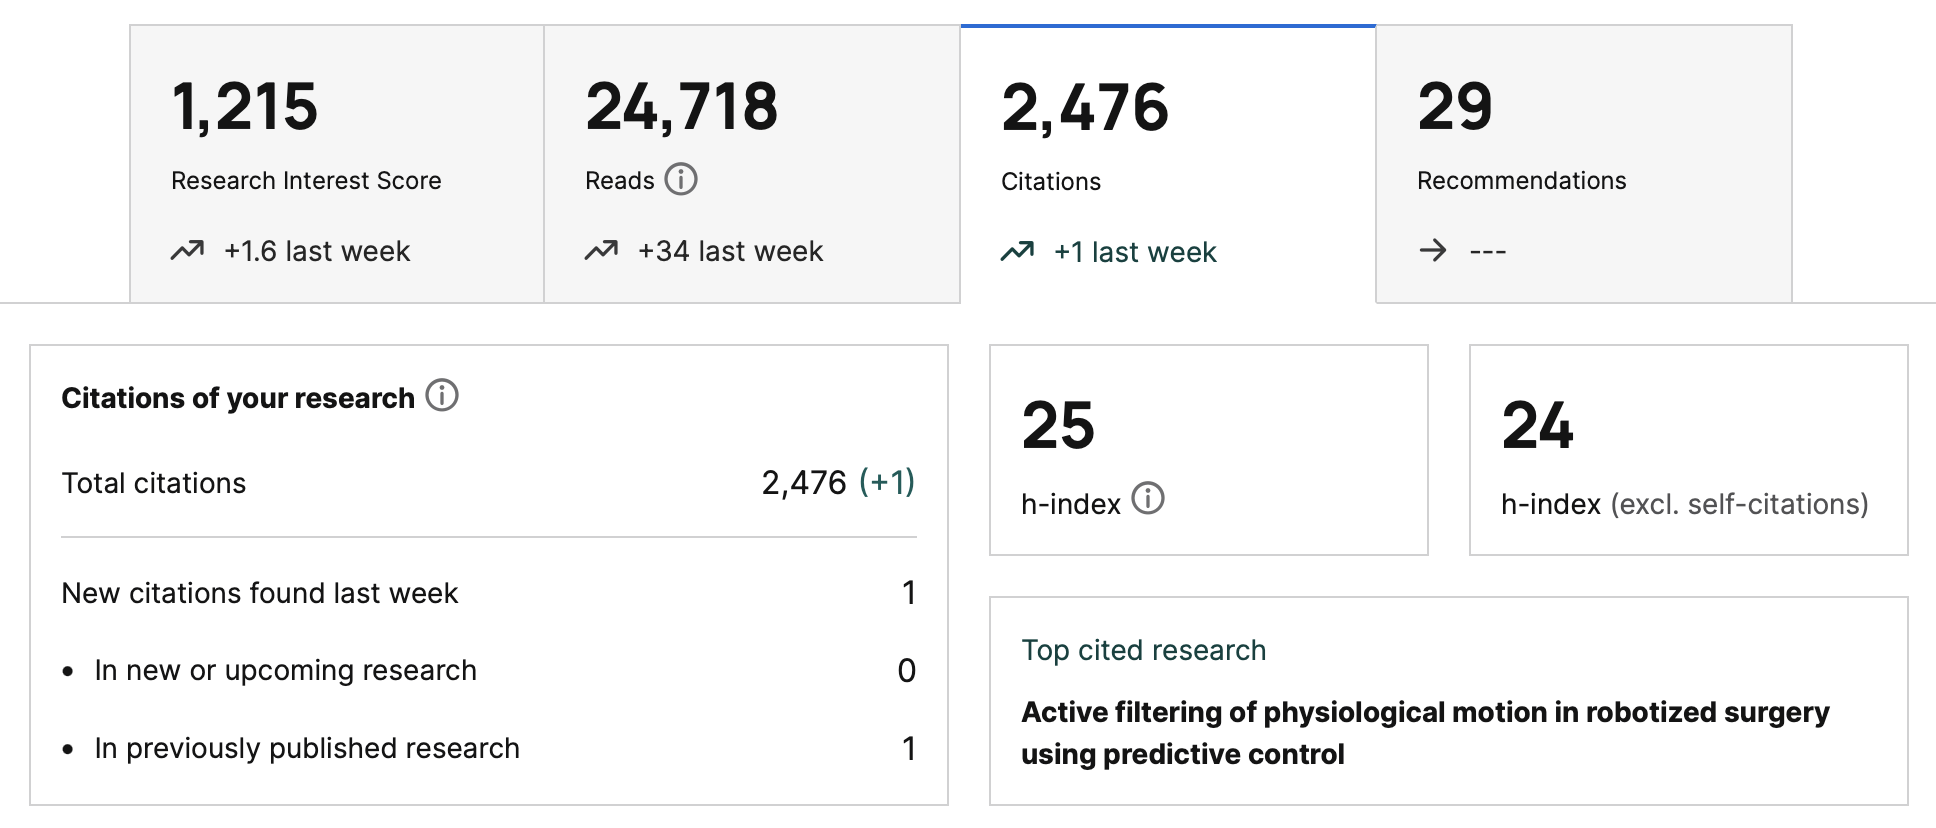
\includegraphics[width=0.7\textwidth]{stats_RG.png}
\caption{Statistiques bibliométriques}
\label{fig:stats}
\end{figure}

Ci-dessous la liste de ce que je considère comme mes 5 principales publications de ces dernières années :
\begin{enumerate}
    \item La publication \cite{2-BCLG19} parue dans \textit{IEEE TRO} en 2019 marque le début de la reconnaissance au plus haut niveau de nos travaux en robotique parallèle à câbles après plusieurs années de travail pour monter en compétences dans ce domaine.
    \item La publication \cite{2-YCAD23} parue dans \textit{IEEE TRO} en 2023 marque quant à elle le le début de la reconnaissance au plus haut niveau de nos travaux en manipulation aérienne.
    \item La publication \cite{2-CAYD23} parue dans \textit{Mechanism and Machine Theory} en 2023 marque  une étape importante de la transition entre la robotique parallèle à câbles et la manipulation aérienne.
    \item Les publications \cite{2-NDCD24} et \cite{2-ANCDxx} parues respectivement en 2024 et 2025 dans \textit{IEEE RAL} confirment notre positionnement sur des thématiques novatrices en manipulation aérienne. 
\end{enumerate}

Je souhaiterais aussi mentionner ici le rôle parfois ingrat du logiciel dans des travaux de recherche qui ont souvent un important volet expérimental. Depuis 2016, j'ai consacré beaucoup de temps à développer trois logiciels libres qui ont fortement dynamisé notre productivité scientifique en permettant un prototypage très rapide des lois de commande testées. C'est un peu la partie immergée de l'iceberg :
\begin{enumerate}
    \item \textbf{RPIt}\footnote{\url{https://github.com/jacqu/rpit}} : une boîte à outils pour le logiciel Simulink qui fournit des blocs permettant de s'interfacer simplement avec nos systèmes et de décrire simplement nos lois de commande sous forme de schéma-bloc. Par exemple, l'un de ces blocs représente toutes les entrées et les sorties accessibles sur un contrôleur de vol de type Betaflight.
    \item \textbf{Betalink}\footnote{\url{https://github.com/jacqu/betalink}} : un firmware de controleur de vol Betaflight modifié pour réguler finement et rapidement la vitesse de rotation des moteurs de drone.
    \item \textbf{Teensyshot}\footnote{\url{https://github.com/jacqu/teensyshot}} : un logiciel embarqué permettant de réguler la vitesse des moteurs de drone connectés à un ESC de marque KISS.
\end{enumerate}

Ces projets sont en accès libre sur ma page GitHub et je suis leur principal contributeur. Certains, comme Teensyshot qui a été co-développé avec Arda Yigit, bénéficient d'une certaine popularité. 

%%%%%%%%%%%%%%%%%%%%%%%%%%%%%%%%%%%%%%%%%%%%%%%%%%%%%%%%%%%%
\subsection{Encadrement doctoral et scientifique}
%%%%%%%%%%%%%%%%%%%%%%%%%%%%%%%%%%%%%%%%%%%%%%%%%%%%%%%%%%%%

Depuis ma dernière promotion, j'ai dirigé 8 thèses, l'une d'entre elles étant encore en cours :

\begin{table}[htbp]
%\caption{Variable Descriptions}
\label{tab:liste_theses}
\centering
\begin{tabular}{>{\bfseries}lll}
\toprule
\textup{\textcolor{orange}{Dates}} & \textcolor{orange}{NOM Prénom} & \textcolor{orange}{Thématique}\\
\midrule
2022 -- & NIDDAM Ethan & Manipulation aérienne\\
2020 -- 2023 & ARPA PEROZO Miguel & Manipulation aérienne\\
2018 -- 2021 & YIGIT Arda & Manipulation aérienne\\
2016 -- 2021 & KHAYOUR Imane & Robotique parallèle à cables\\
2015 -- 2019 & LESELLIER Maximilien & Robotique parallèle à câbles\\
2012 -- 2016 & WEBER Xavier & Robotique parallèle à câbles\\
2009 -- 2012 & RUBBERT Lennart & Robotique médicale\\
2007 -- 2012 & JOINIE-MAURIN Matthieu & Robotique méciale\\
\bottomrule
\end{tabular}
\end{table}

Tous les détails sont donnés dans l'annexe \ref{sec:theses}. En moyenne, mon taux d'encadrement s'élève à 38\% sur la période de référence. En moyenne, mes interactions avec mes doctorants se font avec une périodicité d'une réunion de deux heures par semaine. Je module cette fréquence en fonction du doctorant et/ou de l'état d'avancement de la thèse. Il m'est arrivé de faire des points quotidiens de 30 minutes avec certains doctorants pendant une année entière pour débloquer leur travail de thèse. Je participe activement à la correction de leurs publications et de leur manuscrit de thèse. Je suis assisté par mes collègues. Ces dernières années, j'ai beaucoup travaillé avec Sylvain Durand et Loïc Cuvillon. Loïc en particulier s'est énormément investi dans l'encadrement de ces thèses et je l'en remercie vivement.

Durant la période de référence, j’ai aussi encadré les étudiants en stage de master/fin d’études suivants sur une période de 5 mois :
\begin{itemize}
    \item 2015 : Lyad Hamouchi (100\%), Maximilien Lesellier (100\%)
    \item 2016 : Alice Magissson (30\%)
    \item 2017 : Imane Khayour (100\%), Guillaume Rouault (100\%)
    \item 2018 : Jérémy Begey (70\%)
    \item 2019 : Hugo Sellet (100\%)
    \item 2020 : Yannick Kuhn (30\%), Miguel Arpa Perozo (100\%)
    \item 2021 : Jean Dussine (100\%)
    \item 2022 : Thibaut Lopez (100\%), Ethan Niddam (100\%), Charlotte Leclerc (100\%)
    \item 2023 : Clément Cherbonnel (100\%), Hugo Sébire (100\%)
\end{itemize}

La liste précédente montre que l'encadrement de stagiaires de master est souvent un bon moyen de recruter un doctorant. Ainsi, parmi tous les stagiaires que j'ai encadrés ces dernières années, Maximilien, Imane, Miguel et Ethan ont poursuivi en thèse. Actuellement, je n'encadre plus qu'une seule thèse, celle d'Ethan, qui devrait être soutenue avant la fin de l'année. L'an dernier, je n'ai pas réussi à recruter de thésard sur le sujet que j'avais déposé à l'école doctorale. J'avais recruté un stagiaire de master avec un excellent profil. Malheureusement, il s'est désisté au dernier moment en raison des nouvelles contraintes liées à la procédure FSD. C'est dommage, car je pense que ça aurait été un excellent candidat pour ma thèse. Cette année, je vais multiplier les sujets et les canaux de financement potentiels de thèse : dépôt d'un projet ANR, le PEPR AR et l'école doctorale. J'espère que j'aurai plus de succès.

%%%%%%%%%%%%%%%%%%%%%%%%%%%%%%%%%%%%%%%%%%%%%%%%%%%%%%%%%%%%
\subsection{Diffusion et rayonnement}
%%%%%%%%%%%%%%%%%%%%%%%%%%%%%%%%%%%%%%%%%%%%%%%%%%%%%%%%%%%%

% •	expertise (organismes nationaux ou internationaux)
% •	activités éditoriales (expertises, responsabilités de collections…)
% •	participation jurys de thèse et de HDR (hors établissement)
% •	diffusion du savoir (vulgarisation), responsabilités et activités au sein des sociétés savantes ou associations
% •	organisation colloques, conférences, journées d’étude
% •	participation à un réseau de recherche, invitations dans des universités étrangères…

\subsubsection{Expertise}

Je participe régulièrement à des comités de sélection (environ 1 par an) pour le recrutement de maîtres de conférences ou de professeurs. Les derniers auxquels j'ai participé sont :
\begin{itemize}
    \item 2024 : LIRMM, Montpellier, poste de PU
    \item 2023 : FEMTO-ST, Besançon, poste de PU
    \item 2022 : Université de Nice, repyramidage MCF vers PU
    \item 2021 : LIRMM, Montpellier, poste de MCF
    \item 2020 : ENIM, Metz, poste de PU
\end{itemize}

J'expertise régulièrement des projets ANR (environ 1 par an).

Je participe aussi régulièrement au jury des prix de thèse du GdR robotique (une fois tous les deux ans environ).

De façon plus ponctuelle, j'ai aussi fait une expertise HCERES de formation de master et quelques expertises de projets régionaux.


\subsubsection{Activités éditoriales}

Je suis éditeur associé du journal \textit{IEEE Robotics and Automation Letters} depuis mai 2024. Je consacre environ 4 heures par semaine à cette fonction. La tâche la plus chronophage consiste à trouver des experts pertinents ET volontaires ET disponibles pour des articles qui ne sont parfois pas dans mon domaine de compétences. Le reste du travail consiste à rédiger les recommandations en fonction des avis des experts. J'ai en moyenne 3 articles à gérer en même temps.

Je suis régulièrement éditeur associé des conférences ICRA avec en moyenne 8 articles à gérer : ICRA2020, ICRA2021, ICRA2024 et ICRA2025. J'ai aussi été éditeur associé de la conférence IROS : IROS2014, IROS2015 et IROS2016.

\subsubsection{Participation jurys de thèse et de HdR}

Le tableau ci-dessous dresse la liste de tous les jurys de thèse ou d'HdR auxquels j'ai participé en dehors de mon établissement d'affectation depuis ma dernière promotion. Sur ces 28 jurys, 3 se sont tenus ou vont se tenir (les deux premières lignes sont des jurys à venir) à l'étranger (Skoltech, University of Twente, University of Hong-Kong).
\newline

{\centering
\setlength{\tabcolsep}{2pt} % . The default value is 6pt.
\begin{tabular}{cccccc} \toprule
    \textcolor{orange}{Année} & \textcolor{orange}{Candidat} & \textcolor{orange}{Diplôme} & \textcolor{orange}{Laboratoire} & \textcolor{orange}{Etablissement} & \textcolor{orange}{Fonction} \\ \midrule
2025 & \bf{Sophie ROUSSEAU} & These & IRT Jules Verne & Centrale Nantes & Rapporteur \\
2025 & \bf{Gino INNERO} & These & CUHK & Univ. of Hong-Kong (CN) & Rapporteur \\
2024 & \bf{Marco TOGNON} & HdR & INRIA-RAINBOW & Univ. de Rennes & Rapporteur \\
2024 & \bf{Abir BOUAOUDA} & Thèse & CRAN & Univ. de Lorraine & Président/Rapporteur \\
2024 & \bf{Lev SMOLENTSEV} & Thèse & IRISA & Univ. de Rennes & Président \\
2024 & \bf{Andre FIALHO COELHO}  & Thèse & EEMCS & Univ. of Twente (NL) & Rapporteur \\
2023 & \bf{Jérôme TRUC}  & Thèse & LAAS & Univ. de Toulouse 3 & Examinateur \\
2023 & \bf{Benjamin CALME}  & Thèse & LIRMM & Univ. de Montpellier & Président \\
2022 & \bf{Ghina HASSAN} & Thèse & LIRMM & Univ. de Montpellier & Rapporteur \\
2022 & \bf{Yuri SARKISOV} & Thèse & DLR (DE) & Skoltech (RU) & Rapporteur \\
2022 & \bf{Dario SANALITRO} & Thèse & LAAS & INSA Toulouse & Rapporteur \\ 
2022 & \bf{Carlos Wilfrido PONCE QUIROGA}  & Thèse & LCFC & Univ. de Metz & Président \\
2020 & \bf{João CAVALCANTI SANTOS}  & Thèse & LIRMM & Univ. de Montpellier & Rapporteur \\ 
2020 & \bf{Atal Anil KUMAR}  & Thèse & LCFC & Univ. de Lorraine & Président \\ 
2020 & \bf{Franco FUSCO}  & Thèse & LS2N & Centrale Nantes & Rapporteur \\ 
2019 & \bf{Komlan Yves KOLEGAIN}  & Thèse & LCFC & ENSAM & Rapporteur \\ 
2017 & \bf{Andrey KUDRYAVTSEV}  & Thèse & FEMTO-ST & Univ. de Franche-Comté & Rapporteur \\
2016 & \bf{Marc GOUTTEFARDE}  & HdR & LIRMM & Univ. de Montpellier & Rapporteur \\
2016 & \bf{Victor GIBERT}  & Thèse & IRCCyN & Univ. de Nantes & Rapporteur \\
2016 & \bf{Le CUI}  & Thèse & IRISA & Univ. de Rennes 1 & Rapporteur \\
2015 & \bf{Cédric CLEVY}  & HdR & FEMTO-ST & Univ. de Franche-Comté & Rapporteur \\
2015 & \bf{Han YUAN}  & Thèse & LGCGM & INSA Rennes & Rapporteur \\
2014 & \bf{Omar TAHRI} & HdR & LE2I & Univ. de Bourgogne & Rapporteur \\
2014 & \bf{Dinh Quan NGUYEN}  & Thèse & LIRMM & Univ. de Montpellier 2 & Rapporteur \\
2013 & \bf{Sounkalo DEMBELE}  & HdR & FEMTO-ST & Univ. de Franche-Comté & Examinateur \\
2013 & \bf{Benoît ROSA}  & Thèse & ISIR & Univ. P. et M. Curie & Rapporteur \\
2013 & \bf{Jinna QIN}  & Thèse & LCFC & ENSAM & Rapporteur \\
2013 & \bf{Julien ALEXANDRE DIT SANDRETTO}  & Thèse & INRIA-COPRIN & Univ. de Nice & Rapporteur \\ \bottomrule
\end{tabular}
}

\subsubsection{Diffusion du savoir}

Le 18 juin 2024, j'ai fait une présentation à la conférence sur la sobriété organisée par le réseau Alsace tech à destination du monde socio-économique. Ma présentation, \href{https://youtu.be/kJXx7LR21H4?t=2701}{disponible sur la chaîne YouTube d'Alsace tech} était une rétrospective sur toute ma carrière de ma démarche scientifique, qui tend vers la recherche des systèmes les plus simples et parcimonieux en ressources possibles, pour réaliser une tâche donnée. Le public était essentiellement composé d'industriels locaux.

Le 15 février 2024, j'ai fait une présentation à l'INRIA Rennes en marge de l'HdR de Marco Tognon, retraçant une rétrospective de mes 10 dernières années de recherche sous l'angle de la frugalité. J'ai enregistré cette présentation et je l'ai \href{https://youtu.be/ThW7nigN9hQ}{publiée sur ma chaîne YouTube}.

Le 19 janvier 2024, j'ai fait une présentation générale de mes travaux en lien avec la frugalité à destination de tous mes collègues d'ICube dans le cadre d'animations scientifiques pour les 10 ans du laboratoire.

En juillet 2021, j'ai fait une présentation générale de mes travaux en robotique aérienne au groupe de travail << UAV >> du GdR MACS, de leur genèse jusqu'aux derniers développements.

Je participe régulièrement à la fête de la science où l'équipe tient tous les deux ans un stand qui présente des systèmes robotiques issus de nos recherches.

Je publie régulièrement des vidéos de nos expériences de robotique sur ma chaîne YouTube. Par exemple, \href{https://youtu.be/fZkru3tZsYo}{la dernière} qui porte sur le travail de thèse d'Ethan NIDDAM a recueilli 750 vues en 7 mois.

\subsubsection{Distinctions}

Arda Yigit dont j'ai dirigé la thèse de 2018 à 2021 a obtenu :
\begin{itemize}
    \item le prix du meilleur poster vidéo aux JJCR 2020
    \item le deuxième prix de thèse du GdR robotique en 2022
\end{itemize}

%%%%%%%%%%%%%%%%%%%%%%%%%%%%%%%%%%%%%%%%%%%%%%%%%%%%%%%%%%%%
\subsection{Responsabilités scientifiques}
%%%%%%%%%%%%%%%%%%%%%%%%%%%%%%%%%%%%%%%%%%%%%%%%%%%%%%%%%%%%


% •	Animation équipes de recherche (préciser le rôle, taille, composition, budget)
% •	Contrats de recherche évalués suite à appel à projet (préciser l’organisme, les dates, le rôle, les ressources financières et humaines)
% •	Contrats de recherche de gré à gré (préciser le partenaire, les dates, le rôle, les ressources financières et humaines)

\subsection{Animation}

Je suis animateur du thème << Systèmes complexes et parcimonie >> de mon équipe depuis 2021. L’équipe RDH à laquelle j’appartiens est très grande (51 permanents) et multisite (Hôpital civil et Illkirch). Le thème en question regroupe 12 permanents. Cette mission consiste principalement à organiser des réunions thématiques (une par semestre) et à gérer les problèmes organisationnels propres au site d’Illkirch où est principalement basé ce thème (affectation des bureaux, inventaires des locaux techniques, visites de sécurité, signalétique de sécurité, visites en vue de la création d’une ZRR, implantation de gros équipements, gestion des équipements communs). Ponctuellement, lors de la dernière évaluation HCERES en 2022, cette mission a consisté à animer la réflexion autour de la nouvelle structuration thématique de l’équipe et la prospective du thème en question.

Depuis 2022, je préside le comité d’experts scientifiques de Télécom Physique Strasbourg. Cette mission consiste principalement à entériner les décisions de recrutement des ATER au sein de l’école.

J'ai été animateur de l'axe transverse << Environnement et Développement Durable >> du laboratoire ICube de 2009 à 2013. Cette mission visait à identifier au sein du tout nouveau laboratoire ICube les possibilités de synergies inter-équipes autour de cette thématique. La mission a consisté à animer une dizaine de demi-journées de travail rassemblant une trentaine de participants. Le travail a conduit à la rédaction d'une cartographie des thématiques de recherche potentielles qui a été présentée au comité AERES qui a évalué le laboratoire.

\subsection{Contrats}

\textbf{ANR STRAD (2022 -- 2026)}

\begin{itemize}
    \item Je suis coordinateur de l’ANR STRAD.
    \item Ce projet vise à développer un manipulateur aérien capable de réaliser une oeuvre de street art sur une grande surface verticale.
    \item Budget total : \textbf{440 k€}
    \item Partenaires : Gipsa-lab, Spacejunk Art Centers, Polyvionics, ICube.
    \item Je suis aussi responsable scientifique d'ICube pour ce projet. Le budget alloué pour ICube s'élève à \textbf{218 k€} si on inclut le salaire du doctorant (Ethan NIDDAM) qui est co-encadré par ICube et le Gipsa-lab.
\end{itemize}

\textbf{ANR TIR4sTREEt (2022 -- 2026)}

\begin{itemize}
    \item Je suis responsable du livrable << Drone >> de ce projet avec un budget alloué de \textbf{39 k€}
    \item L’objectif du livrable est de concevoir un manipulateur aérien capable de mouvoir précisément et avec un minimum de perturbations aérodynamiques, des capteurs de climatologie en environnement urbain. 
    \item Deux autres collègues de mon équipe, Sylvain Durand et Loïc Cuvillon, participent aussi à ce livrable. 
    \item Sur le budget total, \textbf{12 k€} sont consacrés aux gratifications de stages.
\end{itemize}

\textbf{ANR eVISER (2018 -- 2021)}
\begin{itemize}
    \item Le projet est du type JCJC.
    \item Coordinateur : Sylvain Durand (ICube)
    \item J'ai participé à ce projet notamment par la direction de la thèse d’Arda Yigit financée par ce projet.
\end{itemize}

\textbf{ANR DexterWide (2015 -- 2019)}
\begin{itemize}
    \item Coordinateur : Marc Gouttefarde, LIRMM
    \item Le projet porte sur l'étude de robots parallèles à câbles dont la plate-forme mobile est équipée d’un ou plusieurs dispositifs actifs permettant l’exécution de tâches dextres sur un vaste espace de travail avec un amortissement rapide des vibrations.
    \item Partenaires : ICube, LIRMM, NFM SYSTEMS, Tecnalia France
    \item J'étais responsable scientifique du partenaire ICube
    \item Budget ICube : \textbf{125k€} dont 1/2 thèse partagée avec le LIRMM
\end{itemize}

% %%%%%%%%%%%%%%%%%%%%%%%%%%%%%%%%%%%%%%%%%%%%%%%%%%%%%%%%%%%%
% \subsection{Autres}
% %%%%%%%%%%%%%%%%%%%%%%%%%%%%%%%%%%%%%%%%%%%%%%%%%%%%%%%%%%%%


%%%%%%%%%%%%%%%%%%%%%%%%%%%%%%%%%%%%%%%%%%%%%%%%%%%%%%%%%%%%
\printbibliography[title={\small Bibliographie de la section << Activités scientifiques >>}]
%%%%%%%%%%%%%%%%%%%%%%%%%%%%%%%%%%%%%%%%%%%%%%%%%%%%%%%%%%%%

%------------------------------------------------------------
\Separation{}
%------------------------------------------------------------


%%%%%%%%%%%%%%%%%%%%%%%%%%%%%%%%%%%%%%%%%%%%%%%%%%%%%%%%%%%%
%%%%%%%%%%%%%%%%%%%%%%%%%%%%%%%%%%%%%%%%%%%%%%%%%%%%%%%%%%%%
\section{Responsabilités collectives et d'intérêt général}
%%%%%%%%%%%%%%%%%%%%%%%%%%%%%%%%%%%%%%%%%%%%%%%%%%%%%%%%%%%%
%%%%%%%%%%%%%%%%%%%%%%%%%%%%%%%%%%%%%%%%%%%%%%%%%%%%%%%%%%%%


% %%%%%%%%%%%%%%%%%%%%%%%%%%%%%%%%%%%%%%%%%%%%%%%%%%%%%%%%%%%%
% \subsection{Présentation synthétique des responsabilités}
% %%%%%%%%%%%%%%%%%%%%%%%%%%%%%%%%%%%%%%%%%%%%%%%%%%%%%%%%%%%%
% 1.	Présentation générale des responsabilités (la rubrique 1 est limitée à 6000 caractères, blancs non compris, soit environ 2 pages) : 


%%%%%%%%%%%%%%%%%%%%%%%%%%%%%%%%%%%%%%%%%%%%%%%%%%%%%%%%%%%%
\subsection{Responsabilités administratives}
%%%%%%%%%%%%%%%%%%%%%%%%%%%%%%%%%%%%%%%%%%%%%%%%%%%%%%%%%%%%
% 2.	Responsabilités administratives
% •	Présidence, vice-présidence d’établissement de l’enseignement supérieur
% •	Direction de composante, d’école doctorale, services communs
% •	Direction de structures de recherche (UMR, EA, ERT, Plateformes …)
% •	Missions et gestion de projets de l’établissement
% •	Autres

J’ai géré de 2020 à 2022 l’acquisition et le financement de la licence campus du logiciel Matlab. Auparavant, l’accès à ce logiciel était géré au moyen de multiples licences de forme hétérogène disséminées au niveau de plusieurs composantes utilisatrices. Mon action a consisté à faire un inventaire de l’utilisation de ce logiciel au niveau de l’ensemble de l’université, à négocier auprès de la société éditrice Mathworks un tarif soutenable pour une licence globale (licence campus), à assurer un transitoire de financement de cette licence en s’appuyant d’abord sur les composantes utilisatrices historiques et finalement à assurer un financement récurrent de cette licence par la direction des services numériques. Le tarif final négocié pour cette licence s'élève à \textbf{65 k€} par an, soit environ la moitié du tarif initialement proposé par Mathworks. À ce jour, près de 3000 personnes utilisent cette licence campus sur toute l’université. J’ai rempli cette mission sans mandat officiel. Étant utilisateur de ce logiciel, j’y avais un intérêt personnel pour l’enseignement et la recherche. Malgré son caractère officieux, cette mission fut particulièrement chronophage, notamment lorsqu’il a fallu convaincre les différents financeurs. Après un transitoire un peu difficile, le financement a été maintenant pérennisé et est assumé entièrement par les services centraux de l'université. En effet, les statistiques globales de son usage lissées sur plusieurs années ont montré que ce logiciel était d'intérêt général pour toute l'université.

%%%%%%%%%%%%%%%%%%%%%%%%%%%%%%%%%%%%%%%%%%%%%%%%%%%%%%%%%%%%
\subsection{Responsabilités et mandats locaux ou régionaux}
%%%%%%%%%%%%%%%%%%%%%%%%%%%%%%%%%%%%%%%%%%%%%%%%%%%%%%%%%%%%
% 3.	Responsabilités et mandats locaux ou régionaux :
% •	Participation aux conseils centraux (rôle, missions, ...)
% •	Participation aux conseils de composantes, de laboratoires…
% •	Autres

Je suis membre élu du collège A du conseil de Telecom Physique Strasbourg depuis 2010. Cette mission consiste principalement à assister aux 3 réunions annuelles, plus quelques réunions extraordinaires, notamment lors des élections du directeur de la composante. Comme je suis aussi coresponsable du master IRIV porté par la composante, je présente au conseil les points à l'ordre du jour concernant le master et qui sont soumis au vote (évolution des maquettes, du règlement des études, convention avec l'INSA, fiche RNCP, modalités et quotas de recrutement sur la plateforme MonMaster, création de nouveaux parcours ...).

Je participe aussi aux conseils restreints chargés de donner un avis sur les dossiers de promotion et je suis régulièrement rapporteur des dossiers de mes collègues. Ce conseil restreint se réunit aussi pour se prononcer sur les profils de postes à faire remonter à l'université.

%%%%%%%%%%%%%%%%%%%%%%%%%%%%%%%%%%%%%%%%%%%%%%%%%%%%%%%%%%%%
\subsection{Responsabilités et mandats (internationaux, nationaux)}
%%%%%%%%%%%%%%%%%%%%%%%%%%%%%%%%%%%%%%%%%%%%%%%%%%%%%%%%%%%%
% 4.	Responsabilités et mandats (internationaux, nationaux)
% •	Participations à des instances nationales - CNU, CNRS…-, conseils des établissements publics, jurys de concours.
% •	Responsabilités exercées dans les Agences Nationales (HCERES, ANR, ...)
% •	Autres :

En 2019, j'ai participé à l'évaluation du master Optique, image, vision, multimédia, champ STS de la ComUE Lyon en tant que chargé d'expertise.

J'ai été membre nommé du CNU en 61e section de 2011 à 2015. Je participais tous les ans aux sessions de qualification aux concours de professeur des universités et aux sessions de promotion.

J'ai participé aux comités d'évaluation AERES des laboratoires ISIR (2012), IBISC (2013) et LISV (2013) en tant qu'expert en robotique.

%------------------------------------------------------------
\Separation{}
%------------------------------------------------------------


% %%%%%%%%%%%%%%%%%%%%%%%%%%%%%%%%%%%%%%%%%%%%%%%%%%%%%%%%%%%%
% %%%%%%%%%%%%%%%%%%%%%%%%%%%%%%%%%%%%%%%%%%%%%%%%%%%%%%%%%%%%
% \section{Autres informations}
% %%%%%%%%%%%%%%%%%%%%%%%%%%%%%%%%%%%%%%%%%%%%%%%%%%%%%%%%%%%%
% %%%%%%%%%%%%%%%%%%%%%%%%%%%%%%%%%%%%%%%%%%%%%%%%%%%%%%%%%%%%

% \instructions{%
% 	{\em
% 		Rubrique pour la présentation de situations particulières ou d'actions non mentionnées précédemment.

% 		\bigskip

% 		Cette rubrique est destinée \textbf{notamment} aux enseignants-chercheurs reconnus travailleurs handicapés (RQTH) pour leur permettre de présenter l'ensemble des activités exercées en compensation de leur handicap.

% 	}
% }


% %------------------------------------------------------------
% \Separation{}
% %------------------------------------------------------------


\newpage
\appendix

%%%%%%%%%%%%%%%%%%%%%%%%%%%%%%%%%%%%%%%%%%%%%%%%%%%%%%%%%%%%
%%%%%%%%%%%%%%%%%%%%%%%%%%%%%%%%%%%%%%%%%%%%%%%%%%%%%%%%%%%%
\section{Annexes}
%%%%%%%%%%%%%%%%%%%%%%%%%%%%%%%%%%%%%%%%%%%%%%%%%%%%%%%%%%%%
%%%%%%%%%%%%%%%%%%%%%%%%%%%%%%%%%%%%%%%%%%%%%%%%%%%%%%%%%%%%


%%%%%%%%%%%%%%%%%%%%%%%%%%%%%%%%%%%%%%%%%%%%%%%%%%%%%%%%%%%%
\subsection{Tableau des enseignements depuis la dernière promotion}
%%%%%%%%%%%%%%%%%%%%%%%%%%%%%%%%%%%%%%%%%%%%%%%%%%%%%%%%%%%%
\label{sec:annexe_enseignements}

%%%%%%%%%%%%%%%%%%%%%%
% 24-25, 23-24, 22-23
%%%%%%%%%%%%%%%%%%%%%%

{\centering
\setlength{\tabcolsep}{2pt} % . The default value is 6pt.

\begin{tabular}{cccccccc} \toprule
    \textcolor{orange}{Année} & \textcolor{orange}{Niveau} & \textcolor{orange}{Diplôme} & \textcolor{orange}{Intitulé} & \textcolor{orange}{Type} & \textcolor{orange}{Nature} & \textcolor{orange}{Effectifs} & \textcolor{orange}{Volume (HTD)} \\ \midrule
 \bf{24-25} & 2e année  & Ingénieur & Robotique et automatisme & FISE & CM & 93 & 5,25 \\
 $\cdot$ & 2e année  & Ingénieur & Ingénierie durable  & FISE & CM,Projet & 13  & 46,125  \\
  $\cdot$ & 2e année  & Ingénieur & Commande numérique  & FISE & CM,TP & 17  & 31,75  \\
  $\cdot$ & 3e année  & Ingénieur & Drone : conception, fabrication et commande & FISE & CM,TP & 23 & 14,875  \\
  $\cdot$ & 3e année  & Ingénieur & Robotique appliquée  & FISE & TP & 10  & 12  \\
  $\cdot$ & 3e année  & Ingénieur & Asservissements visuels rapides & FISE & CM,TP & 23 & 14,875  \\
  $\cdot$ & 3e année  & Ingénieur & Robotique : manipulation et commande & FISE & CM,TP & 30 & 33,25  \\
  $\cdot$ & 3e année  & Ingénieur & Temps-réel et systèmes embarqués & FISE & CM,TP & 10 & 22,5  \\
  $\cdot$ & M2        & Master    & Initiation à la recherche & FISE & CM & 81 & 7,875  \\
  $\cdot$ & N/A       & N/A       & Responsabilité parcours de master & N/A & N/A & N/A & 6  \\
  $\cdot$ & N/A       & N/A       & Responsabilité direction de master & N/A & N/A & N/A & 25  \\ 
 \bf{Total} & $\cdot$ & $\cdot$ & $\cdot$ & $\cdot$ & $\cdot$ & $\cdot$ &  {\bf 219,5} \\\midrule
  \bf{23-24} & 2e année  & Ingénieur & Robotique et automatisme & FISE & CM & 76 & 5,25 \\
 $\cdot$ & 2e année  & Ingénieur & Ingénierie durable  & FISE & CM,Projet & 11  & 46,125  \\
  $\cdot$ & 2e année  & Ingénieur & Commande numérique  & FISE & CM,TP & 13  & 29,125  \\
  $\cdot$ & 3e année  & Ingénieur & Drone : conception, fabrication et commande & FISE & CM,TP & 24 & 15,75  \\
  $\cdot$ & 3e année  & Ingénieur & Robotique appliquée  & FISE & TP & 10  & 4  \\
  $\cdot$ & 3e année  & Ingénieur & Asservissements visuels rapides & FISE & CM,TP & 24 & 14,875  \\
  $\cdot$ & 3e année  & Ingénieur & Robotique : manipulation et commande & FISE & CM,TP & 41 & 32,875  \\
  $\cdot$ & 3e année  & Ingénieur & Temps-réel et systèmes embarqués & FISE & CM,TP & 10 & 22,5  \\
  $\cdot$ & M2        & Master    & Initiation à la recherche & FISE & CM & 107 & 7,875  \\
  $\cdot$ & N/A       & N/A       & Responsabilité parcours de master & N/A & N/A & N/A & 6  \\
  $\cdot$ & N/A       & N/A       & Responsabilité direction de master & N/A & N/A & N/A & 25  \\
  $\cdot$ & N/A       & N/A       & Mission référentiel compétences & N/A & N/A & N/A & 8  \\ 
 \bf{Total} & $\cdot$ & $\cdot$ & $\cdot$ & $\cdot$ & $\cdot$ & $\cdot$ &  {\bf 217,4} \\\midrule
\bf{22-23} & 2e année  & Ingénieur & Robotique et automatisme & FISE & CM & 93 & 5,25 \\
 $\cdot$ & 2e année  & Ingénieur & Ingénierie durable  & FISE & CM,Projet & 9  & 50,125  \\
  $\cdot$ & 2e année  & Ingénieur & Commande numérique  & FISE & CM,TP & 14  & 31,75  \\
  $\cdot$ & 3e année  & Ingénieur & Vision et commande & FISE & CM,TP & 26 & 15,75  \\
  $\cdot$ & 3e année  & Ingénieur & Robotique : manipulation et commande & FISE & CM,TP & 38 & 32,25  \\
  $\cdot$ & 3e année  & Ingénieur & Temps-réel et systèmes embarqués & FISE & CM,TP & 13 & 22,5  \\
  $\cdot$ & 3e année  & Ingénieur & Technologie des asservissements & FISE & CM & 13 & 5,25  \\
  $\cdot$ & 3e année  & Ingénieur & Projets tutorés & FISE & Projet & 2 & 10  \\
  $\cdot$ & M2        & Master    & Initiation à la recherche & FISE & CM & 107 & 7,875  \\
  $\cdot$ & N/A       & N/A       & Responsabilité parcours de master & N/A & N/A & N/A & 6  \\
  $\cdot$ & N/A       & N/A       & Responsabilité direction de master & N/A & N/A & N/A & 25  \\
  \bf{Total} & $\cdot$ & $\cdot$ & $\cdot$ & $\cdot$ & $\cdot$ & $\cdot$ &  {\bf 212} \\ \bottomrule
\end{tabular}

}

%%%%%%%%%%%%%%%%%%%%%%
% 21-22, 20-21, 19-20
%%%%%%%%%%%%%%%%%%%%%%
\newpage

{\centering
\setlength{\tabcolsep}{2pt} % . The default value is 6pt.

\begin{tabular}{cccccccc} \toprule
    \textcolor{orange}{Année} & \textcolor{orange}{Niveau} & \textcolor{orange}{Diplôme} & \textcolor{orange}{Intitulé} & \textcolor{orange}{Type} & \textcolor{orange}{Nature} & \textcolor{orange}{Effectifs} & \textcolor{orange}{Volume (HTD)} \\ \midrule
 \bf{21-22} & 2e année  & Ingénieur & Robotique et automatisme & FISE & CM & 80 & 13,25 \\
 $\cdot$ & 2e année  & Ingénieur & Ingénierie durable  & FISE & CM,Projet & 22  & 50,125  \\
  $\cdot$ & 2e année  & Ingénieur & Commande numérique  & FISE & CM,TP & 34  & 31,75  \\
  $\cdot$ & 3e année  & Ingénieur & Vision et commande & FISE & CM,TP & 32 & 15,75  \\
  $\cdot$ & 3e année  & Ingénieur & Robotique : manipulation et commande & FISE & CM,TP & 48 & 32.25  \\
  $\cdot$ & 3e année  & Ingénieur & Temps-réel et systèmes embarqués & FISE & CM,TP & 14 & 22,5  \\
  $\cdot$ & 3e année  & Ingénieur & Technologie des asservissements & FISE & CM & 14 & 5,25  \\
  $\cdot$ & M2        & Master    & Initiation à la recherche & FISE & CM & 93 & 7,875  \\
  $\cdot$ & N/A       & N/A       & Responsabilité parcours de master & N/A & N/A & N/A & 6  \\
  $\cdot$ & N/A       & N/A       & Responsabilité direction de master & N/A & N/A & N/A & 25  \\
  $\cdot$ & N/A       & N/A       & Responsabilité de département & N/A & N/A & N/A & 50  \\
 \bf{Total} & $\cdot$ & $\cdot$ & $\cdot$ & $\cdot$ & $\cdot$ & $\cdot$ &  {\bf 260} \\\midrule
  \bf{20-21} & 2e année  & Ingénieur & Robotique et automatisme & FISE & CM & 99 & 13,25 \\
 $\cdot$ & 2e année  & Ingénieur & Ingénierie durable  & FISE & CM,Projet & 12  & 50,125  \\
  $\cdot$ & 2e année  & Ingénieur & Commande numérique  & FISE & CM,TP & 41  & 31,75  \\
  $\cdot$ & 3e année  & Ingénieur & Vision et commande & FISE & CM,TP & 43 & 15,75  \\
  $\cdot$ & 3e année  & Ingénieur & Robotique : manipulation et commande & FISE & CM,TP & 63 & 32.25  \\
  $\cdot$ & 3e année  & Ingénieur & Temps-réel et systèmes embarqués & FISE & CM,TP & 20 & 22,5  \\
  $\cdot$ & 3e année  & Ingénieur & Technologie des asservissements & FISE & CM & 20 & 7,875  \\
  $\cdot$ & M2        & Master    & Initiation à la recherche & FISE & CM & 108 & 7,875  \\
  $\cdot$ & N/A       & N/A       & Responsabilité parcours de master & N/A & N/A & N/A & 6  \\
  $\cdot$ & N/A       & N/A       & Responsabilité direction de master & N/A & N/A & N/A & 25  \\
  $\cdot$ & N/A       & N/A       & Responsabilité de département & N/A & N/A & N/A & 50  \\
 \bf{Total} & $\cdot$ & $\cdot$ & $\cdot$ & $\cdot$ & $\cdot$ & $\cdot$ &  {\bf 262,4} \\\midrule
  \bf{19-20} & 2e année  & Ingénieur & Robotique et automatisme & FISE & CM & 101 & 13,25 \\
 $\cdot$ & 2e année  & Ingénieur & Ingénierie durable  & FISE & CM,Projet & 18  & 50,125  \\
  $\cdot$ & 2e année  & Ingénieur & Commande numérique  & FISE & CM,TP & 59  & 31,75  \\
  $\cdot$ & 3e année  & Ingénieur & Vision et commande & FISE & CM,TP & 44 & 15,75  \\
  $\cdot$ & 3e année  & Ingénieur & Robotique : manipulation et commande & FISE & CM,TP & 64 & 32.25  \\
  $\cdot$ & 3e année  & Ingénieur & Temps-réel et systèmes embarqués & FISE & CM,TP & 15 & 22,5  \\
  $\cdot$ & 3e année  & Ingénieur & Technologie des asservissements & FISE & CM & 15 & 5.25  \\
  $\cdot$ & N/A       & N/A       & Responsabilité parcours de master & N/A & N/A & N/A & 6  \\
  $\cdot$ & N/A       & N/A       & Responsabilité direction de master & N/A & N/A & N/A & 25  \\
  $\cdot$ & N/A       & N/A       & Responsabilité de département & N/A & N/A & N/A & 50  \\
  \bf{Total} & $\cdot$ & $\cdot$ & $\cdot$ & $\cdot$ & $\cdot$ & $\cdot$ &  {\bf 252} \\ \bottomrule
\end{tabular}

}

%%%%%%%%%%%%%%%%%%%%%%
% 16-17, 17-18, 18-19
%%%%%%%%%%%%%%%%%%%%%%
\newpage

{\centering
\setlength{\tabcolsep}{2pt} % . The default value is 6pt.

\begin{tabular}{cccccccc} \toprule
    \textcolor{orange}{Année} & \textcolor{orange}{Niveau} & \textcolor{orange}{Diplôme} & \textcolor{orange}{Intitulé} & \textcolor{orange}{Type} & \textcolor{orange}{Nature} & \textcolor{orange}{Effectifs} & \textcolor{orange}{Volume (HTD)} \\ \midrule
 \bf{18-19} & 2e année  & Ingénieur & Robotique et automatisme & FISE & CM & 91 & 13,25 \\
 $\cdot$ & 2e année  & Ingénieur & Ingénierie durable  & FISE & CM,Projet & 13  & 50,125  \\
  $\cdot$ & 2e année  & Ingénieur & Commande numérique  & FISE & CM,TP & 49  & 31,75  \\
  $\cdot$ & 3e année  & Ingénieur & Vision et commande & FISE & CM,TP & 32 & 15,75  \\
  $\cdot$ & 3e année  & Ingénieur & Robotique : manipulation et commande & FISE & CM,TP & 44 & 29,7  \\
  $\cdot$ & 3e année  & Ingénieur & Temps-réel et systèmes embarqués & FISE & CM,TP & 15 & 22,5  \\
  $\cdot$ & 3e année  & Ingénieur & Technologie des asservissements & FISE & CM & 15 & 5,25  \\
  $\cdot$ & N/A       & N/A       & Responsabilité parcours de master & N/A & N/A & N/A & 6  \\
  $\cdot$ & N/A       & N/A       & Responsabilité direction de master & N/A & N/A & N/A & 25  \\
  $\cdot$ & N/A       & N/A       & Responsabilité de département & N/A & N/A & N/A & 50  \\
 \bf{Total} & $\cdot$ & $\cdot$ & $\cdot$ & $\cdot$ & $\cdot$ & $\cdot$ &  {\bf 250} \\\midrule
  \bf{17-18} & 2e année  & Ingénieur & Robotique et automatisme & FISE & CM & 72 & 21,25 \\
 $\cdot$ & 2e année  & Ingénieur & Ingénierie durable  & FISE & CM,Projet & 13  & 50,125  \\
  $\cdot$ & 2e année  & Ingénieur & Commande numérique  & FISE & CM,TP & 56  & 15  \\
  $\cdot$ & 3e année  & Ingénieur & Vision et commande & FISE & CM,TP & 35 & 15,75  \\
  $\cdot$ & 3e année  & Ingénieur & Robotique : manipulation et commande & FISE & CM,TP & 48 & 29  \\
  $\cdot$ & 3e année  & Ingénieur & Temps-réel et systèmes embarqués & FISE & CM,TP & 16 & 22,5  \\
  $\cdot$ & 3e année  & Ingénieur & Technologie des asservissements & FISE & CM & 16 & 5.25  \\
  $\cdot$ & 3e année  & Ingénieur & Technologies vertes & FISE & CM & 16 & 7,875  \\
  $\cdot$ & N/A       & N/A       & Responsabilité parcours de master & N/A & N/A & N/A & 6  \\
  $\cdot$ & N/A       & N/A       & Responsabilité direction de master & N/A & N/A & N/A & 25  \\
  $\cdot$ & N/A       & N/A       & Responsabilité de département & N/A & N/A & N/A & 50  \\
 \bf{Total} & $\cdot$ & $\cdot$ & $\cdot$ & $\cdot$ & $\cdot$ & $\cdot$ &  {\bf 247,3} \\\midrule
  \bf{16-17} & 2e année  & Ingénieur & Robotique et automatisme & FISE & CM & 77 & 21,25 \\
 $\cdot$ & 2e année  & Ingénieur & Ingénierie durable  & FISE & CM,Projet & 16  & 50,125  \\
  $\cdot$ & 2e année  & Ingénieur & Commande numérique  & FISE & CM,TP & 57  & 15  \\
  $\cdot$ & 3e année  & Ingénieur & Vision et commande & FISE & CM,TP & 29 & 15,75  \\
  $\cdot$ & 3e année  & Ingénieur & Robotique : manipulation et commande & FISE & CM,TP & 44 & 29  \\
  $\cdot$ & 3e année  & Ingénieur & Temps-réel et systèmes embarqués & FISE & CM,TP & 22 & 22,5  \\
  $\cdot$ & 3e année  & Ingénieur & Technologie des asservissements & FISE & CM & 22 & 5.25  \\
  $\cdot$ & 3e année  & Ingénieur & Technologies vertes & FISE & CM & 22 & 7,875  \\
  $\cdot$ & 3e année  & Ingénieur & Commande optimale & FISE & CM & 22 & 7,875  \\
  $\cdot$ & 3e année  & Ingénieur & Projets tutorés & FISE & Projet & 2 & 10  \\
  $\cdot$ & N/A       & N/A       & Responsabilité parcours de master & N/A & N/A & N/A & 6  \\
  $\cdot$ & N/A       & N/A       & Responsabilité direction de master & N/A & N/A & N/A & 25  \\
  $\cdot$ & N/A       & N/A       & Responsabilité de département & N/A & N/A & N/A & 15  \\
  \bf{Total} & $\cdot$ & $\cdot$ & $\cdot$ & $\cdot$ & $\cdot$ & $\cdot$ &  {\bf 230,6} \\ \bottomrule
\end{tabular}

}

%%%%%%%%%%%%%%%%%%%%%%
% 13-14, 14-15, 15-16
%%%%%%%%%%%%%%%%%%%%%%
\newpage

{\centering
\setlength{\tabcolsep}{2pt} % . The default value is 6pt.

\begin{tabular}{cccccccc} \toprule
    \textcolor{orange}{Année} & \textcolor{orange}{Niveau} & \textcolor{orange}{Diplôme} & \textcolor{orange}{Intitulé} & \textcolor{orange}{Type} & \textcolor{orange}{Nature} & \textcolor{orange}{Effectifs} & \textcolor{orange}{Volume (HTD)} \\ \midrule
  \bf{15-16} & 2e année  & Ingénieur & Robotique et automatisme & FISE & CM & 80 & 21,25 \\
 $\cdot$ & 2e année  & Ingénieur & Ingénierie durable  & FISE & CM,Projet & 24  & 50,125  \\
  $\cdot$ & 2e année  & Ingénieur & Commande numérique  & FISE & CM,TP & 61  & 31,75  \\
  $\cdot$ & 3e année  & Ingénieur & Vision et commande & FISE & CM,TP & 29 & 15,75  \\
  $\cdot$ & 3e année  & Ingénieur & Robotique : manipulation et commande & FISE & CM,TP & 44 & 29  \\
  $\cdot$ & 3e année  & Ingénieur & Temps-réel et systèmes embarqués & FISE & CM,TP & 18 & 22,5  \\
  $\cdot$ & 3e année  & Ingénieur & Technologie des asservissements & FISE & CM & 18 & 5.25  \\
  $\cdot$ & 3e année  & Ingénieur & Technologies vertes & FISE & CM & 18 & 7,875  \\
  $\cdot$ & 3e année  & Ingénieur & Commande optimale & FISE & CM & 18 & 7,875  \\
  $\cdot$ & 3e année  & Ingénieur & Projets tutorés & FISE & Projet & 2 & 10  \\
  $\cdot$ & N/A       & N/A       & Responsabilité parcours de master & N/A & N/A & N/A & 6  \\
  $\cdot$ & N/A       & N/A       & Responsabilité direction de master & N/A & N/A & N/A & 25  \\
  $\cdot$ & N/A       & N/A       & Responsabilité de département & N/A & N/A & N/A & 15  \\
 \bf{Total} & $\cdot$ & $\cdot$ & $\cdot$ & $\cdot$ & $\cdot$ & $\cdot$ &  {\bf 247,4} \\\midrule
  \bf{14-15} & 2e année  & Ingénieur & Robotique et automatisme & FISE & CM & \(\sim \)80 & 21,25 \\
 $\cdot$ & 2e année  & Ingénieur & Ingénierie durable  & FISE & CM,Projet & 31  & 50,125  \\
  $\cdot$ & 2e année  & Ingénieur & Commande numérique  & FISE & CM,TP & 36  & 31,75  \\
  $\cdot$ & 3e année  & Ingénieur & Vision et commande & FISE & CM,TP & 31 & 15,75  \\
  $\cdot$ & 3e année  & Ingénieur & Robotique : manipulation et commande & FISE & CM,TP & 42 & 29  \\
  $\cdot$ & 3e année  & Ingénieur & Temps-réel et systèmes embarqués & FISE & CM,TP & \(\sim \)15 & 22,5  \\
  $\cdot$ & 3e année  & Ingénieur & Technologie des asservissements & FISE & CM & \(\sim \)15 & 5.25  \\
  $\cdot$ & 3e année  & Ingénieur & Technologies vertes & FISE & CM & \(\sim \)15 & 7,875  \\
  $\cdot$ & 3e année  & Ingénieur & Commande optimale & FISE & CM & \(\sim \)15 & 7,875  \\
  $\cdot$ & 3e année  & Ingénieur & Projets tutorés & FISE & Projet & 4 & 20  \\
  $\cdot$ & N/A       & N/A       & Responsabilité de département & N/A & N/A & N/A & 15  \\
 \bf{Total} & $\cdot$ & $\cdot$ & $\cdot$ & $\cdot$ & $\cdot$ & $\cdot$ &  {\bf 226,4} \\\midrule
  \bf{13-14} & 2e année  & Ingénieur & Robotique et automatisme & FISE & CM & \(\sim \)80 & 21,25 \\
 $\cdot$ & 2e année  & Ingénieur & Ingénierie durable  & FISE & CM,Projet & 22  & 50,125  \\
  $\cdot$ & 2e année  & Ingénieur & Commande numérique  & FISE & CM,TP & 33  & 31,75  \\
  $\cdot$ & 3e année  & Ingénieur & Vision et commande & FISE & CM,TP & 24 & 15,75  \\
  $\cdot$ & 3e année  & Ingénieur & Robotique : manipulation et commande & FISE & CM,TP & 36 & 29  \\
  $\cdot$ & 3e année  & Ingénieur & Temps-réel et systèmes embarqués & FISE & CM,TP & 11 & 22,5  \\
  $\cdot$ & 3e année  & Ingénieur & Technologie des asservissements & FISE & CM & 11 & 5.25  \\
  $\cdot$ & 3e année  & Ingénieur & Technologies vertes & FISE & CM & 11 & 7,875  \\
  $\cdot$ & 3e année  & Ingénieur & Commande optimale & FISE & CM & 11 & 7,875  \\
  $\cdot$ & 3e année  & Ingénieur & Projets tutorés & FISE & Projet & 4 & 20  \\
  $\cdot$ & N/A       & N/A       & Responsabilités de missions niveau master & N/A & N/A & N/A & 40  \\
  \bf{Total} & $\cdot$ & $\cdot$ & $\cdot$ & $\cdot$ & $\cdot$ & $\cdot$ &  {\bf 251} \\ \bottomrule
\end{tabular}

}

%%%%%%%%%%%%%%%%%%%%%%
% 12-13
%%%%%%%%%%%%%%%%%%%%%%
\newpage

{\centering
\setlength{\tabcolsep}{2pt} % . The default value is 6pt.

\begin{tabular}{cccccccc} \toprule
    \textcolor{orange}{Année} & \textcolor{orange}{Niveau} & \textcolor{orange}{Diplôme} & \textcolor{orange}{Intitulé} & \textcolor{orange}{Type} & \textcolor{orange}{Nature} & \textcolor{orange}{Effectifs} & \textcolor{orange}{Volume (HTD)} \\ \midrule
  \bf{12-13} & 2e année  & Ingénieur & Robotique et automatisme & FISE & CM & \(\sim \)80 & 21,25 \\
 $\cdot$ & 2e année  & Ingénieur & Ingénierie durable  & FISE & CM,Projet & 18  & 50,125  \\
  $\cdot$ & 2e année  & Ingénieur & Commande numérique  & FISE & CM,TP & 23  & 31,75  \\
  $\cdot$ & 3e année  & Ingénieur & Vision et commande & FISE & CM,TP & 17 & 15,75  \\
  $\cdot$ & 3e année  & Ingénieur & Robotique : manipulation et commande & FISE & CM,TP & 30 & 29  \\
  $\cdot$ & 3e année  & Ingénieur & Temps-réel et systèmes embarqués & FISE & CM,TP & 9 & 22,5  \\
  $\cdot$ & 3e année  & Ingénieur & Technologie des asservissements & FISE & CM & 9 & 5.25  \\
  $\cdot$ & 3e année  & Ingénieur & Technologies vertes & FISE & CM & 9 & 7,875  \\
  $\cdot$ & 3e année  & Ingénieur & Commande optimale & FISE & CM & 9 & 7,875  \\
  $\cdot$ & 3e année  & Ingénieur & Projets tutorés & FISE & Projet & 4 & 20  \\
  $\cdot$ & N/A       & N/A       & Responsabilités de missions niveau master & N/A & N/A & N/A & 35  \\
  \bf{Total} & $\cdot$ & $\cdot$ & $\cdot$ & $\cdot$ & $\cdot$ & $\cdot$ &  {\bf 246} \\ \bottomrule
\end{tabular}

}

\newpage

%%%%%%%%%%%%%%%%%%%%%%%%%%%%%%%%%%%%%%%%%%%%%%%%%%%%%%%%%%%%
\subsection{Liste classée des publications}
%%%%%%%%%%%%%%%%%%%%%%%%%%%%%%%%%%%%%%%%%%%%%%%%%%%%%%%%%%%%

\newrefsection
\nocite{2-ANCDxx,2-NDCD24,2-CAYD23,2-YCAD23,2-YACD21,2-CWG20,2-BCLG19,2-RRCG14,2-BMGB14,2-RCGR14,3-GPLD14,2-GBMN13,2-CLGD12,2-GPLD12,3-NLCG12,3-BLRG12,2-BRLF11,2-BRLG11,2-RRBG11,2-BRCL09,2-BRLF08,2-MBPG08,2-MHIG06,2-RGD06,2-CGDF06,2-GGDS06,2-GGDS05,2-GD03,2-KGDD03,2-GD02,2-SDAG99,}
\printbibliography[title={\small Revues internationales avec comité de lecture}]

\newrefsection
\nocite{1-Gang17,1-GBRP14,1-BJBG14,1-GNP13,1-GNP12,1-BRHG10,1-GP07}
\printbibliography[title={\small Chapitres d'ouvrages}]

\newrefsection
\nocite{10-DMBG05,10-DMBG04,soft_rpit,soft_betalink,soft_teensyshot,soft_luaq}
\printbibliography[title={\small Brevets, licences, logiciels}]

\newrefsection
\nocite{4-LMKN24,4-ADYC22,4-YAOC21,4-YACD21,4-YACD21a,4-KCBY20,4-YGCD20,4-KDCG20,4-SKCD19,4-LCGG18,4-WCG15,4-WCG14,5-CCLG13,5-RRCG13,4-CLCG12,4-LCCG12,4-RRG12a,4-RRG12,4-RCRG12,4-NKG11,4-GPLD11,4-JBG11,5-GPLG11,5-NLCG11,5-GPLD11,4-JRBP10,4-GLPG10,4-GPLG10,7-GPLG10,7-GLPG10,4-GPLG09,4-GLPG09,4-JBBG09,4-BRLG09,7-JBBG09,7-BLRG09,4-ABGG08,4-BLRG08,4-OZND08,5-BLRG08,4-ANBG07,4-BRLG07,4-BRLF07,4-ABAB07,4-BBPG07,4-RCGV07,5-ABGG07,5-ANBG07,7-BRLG07,7-GGP07,7-ANBG07,4-LCGD06,4-MBGP06,4-CLGG06,7-CLGD06,4-CGDF05,4-CLGD05,4-MHGD05,4-MDGB05a,5-MDGB05,4-MGBD04,4-CGLG04,4-MPBG04a,4-MPBG04,4-GGDS04,4-MBBZ04,4-GGDS04a,4-GGDS03c,4-GGDS03,4-GGDS03b,4-CLGD03,4-GGDS03a,5-GGDS03,5-CLGD03,4-MGD02,4-KDGD02a,4-KDDG02,4-GKGD02,4-KDGD02b,4-KDGD02,4-KGDD02,4-KDGD02c,5-KDDG02,4-KDDG01,4-KDGD00,4-GD00,4-GDA99a,4-GDA99}
\printbibliography[title={\small Conférences internationales avec comité de lecture}]



\newpage
%%%%%%%%%%%%%%%%%%%%%%%%%%%%%%%%%%%%%%%%%%%%%%%%%%%%%%%%%%%%
\subsection{Liste des direction et codirection de thèses}
%%%%%%%%%%%%%%%%%%%%%%%%%%%%%%%%%%%%%%%%%%%%%%%%%%%%%%%%%%%%
\label{sec:theses}

\subsubsection{Thèse en cours}

%
% ETHAN
%
\begin{table}[htbp]
%\caption{Variable Descriptions}
\label{tab:Ethan}
\centering
\begin{tabular}{>{\bfseries}ll}
\toprule
\textup{\textcolor{orange}{NOM Prénom}} & \large{\textcolor{orange}{NIDDAM Ethan}}\\
\midrule
Date de début               & Octobre 2022\\
Taux de coencadrement       & 80\%\\
Co-encadrants               & Loïc Cuvillon, Ahmad Hably, Jonathan Dumon, Sylvain Durand\\
Publications                & \emph{Revues} : 2 RAL; \emph{Confs} : 1 ICRA (associée au RAL)\\
\bottomrule
\end{tabular}
\end{table}

\newrefsection
\nocite{2-ANCDxx,2-NDCD24,2-NDCD24-ICRA}
\printbibliography[title={\small Publications du doctorant}]

\newpage
\subsubsection{Thèses soutenues depuis la dernière promotion}

%
% MIGUEL
%
\begin{table}[htbp]
%\caption{Variable Descriptions}
\label{tab:Miguel}
\centering
\begin{tabular}{>{\bfseries}ll}
\toprule % replaced all \hline commands with rules from the booktabs package
\textup{\textcolor{orange}{NOM Prénom}} & \large{\textcolor{orange}{ARPA PEROZO Miguel}}\\
\midrule
Date de début               & Octobre 2020\\
Date de fin                 & Novembre 2023\\
Taux de coencadrement       & 35\%\\
Co-encadrants               & Loïc Cuvillon, Sylvain Durand\\
Publications                & \emph{Revues} : 2 RAL, 1 TRO, 1 MMT; \emph{Confs} : 3 ICRA, 1 IROS\\
Devenir du docteur          & Ingénieur contractuel au Gipsa-lab\\
\bottomrule
\end{tabular}
\end{table}

\newrefsection
\nocite{2-ANCDxx,2-CAYD23,2-YCAD23,4-ADYC22,2-YACD21,4-YAOC21,4-YACD21,4-YACD21a}
\printbibliography[title={\small Publications du doctorant}]

\separation{}

\newpage
%
% ARDA
%
\begin{table}[htbp]
%\caption{Variable Descriptions}
\label{tab:Arda}
\centering
\begin{tabular}{>{\bfseries}ll}
\toprule % replaced all \hline commands with rules from the booktabs package
\textup{\textcolor{orange}{NOM Prénom}} & \large{\textcolor{orange}{YIGIT Arda}}\\
\midrule
Date de début               & Octobre 2018\\
Date de fin                 & Décembre 2021\\
Taux de coencadrement       & 25\%\\
Co-encadrants               & Loïc Cuvillon, Sylvain Durand\\
Publications                & \emph{Revues} : 1 TRO, 1 MMT, 1 RAL; \emph{Confs} : 4 ICRA, 2 IROS \\
Devenir du docteur          & CR CNRS au LS2N\\
\bottomrule
\end{tabular}
\end{table}

\newrefsection
\nocite{2-CAYD23,2-YCAD23,4-ADYC22,2-YACD21,4-YAOC21,4-YACD21,4-YACD21a,4-KCBY20,4-YGCD20,soft_teensyshot}
\printbibliography[title={\small Publications du doctorant}]

\separation{}

\newpage
%
% IMANE
%
\begin{table}[htbp]
%\caption{Variable Descriptions}
\label{tab:Imane}
\centering
\begin{tabular}{>{\bfseries}ll}
\toprule % replaced all \hline commands with rules from the booktabs package
\textup{\textcolor{orange}{NOM Prénom}} & \large{\textcolor{orange}{KHAYOUR Imane}}\\
\midrule
Date de début               & Octobre 2016\\
Date de fin                 & Septembre 2021\\
Taux de coencadrement       & 25\%\\
Co-encadrants               & Loïc Cuvillon, Sylvain Durand\\
Publications                & \emph{Confs} : 1 ICRA, 1 IROS, 1 IFAC WC \\
Devenir du docteur          & CDI Software Application Engineer, Volvo Trucks, Suède\\
\bottomrule
\end{tabular}
\end{table}

\newrefsection
\nocite{4-KCBY20,4-KDCG20,4-SKCD19}
\printbibliography[title={\small Publications du doctorant}]

\separation{}

\newpage
%
% MAXIMILIEN
%
\begin{table}[htbp]
%\caption{Variable Descriptions}
\label{tab:Maximilien}
\centering
\begin{tabular}{>{\bfseries}ll}
\toprule % replaced all \hline commands with rules from the booktabs package
\textup{\textcolor{orange}{NOM Prénom}} & \large{\textcolor{orange}{LESELLIER Maximilien}}\\
\midrule
Date de début               & Décembre 2015\\
Date de fin                 & Février 2019\\
Taux de coencadrement       & 25\%\\
Co-encadrants               & Loïc Cuvillon, Marc Gouttefarde\\
Publications                & \emph{Revue} : 1 TRO; \emph{Conf} : 1 IROS \\
Devenir du docteur          & Directeur général des services adjoint de l'université des Antilles\\
\bottomrule
\end{tabular}
\end{table}

\newrefsection
\nocite{2-BCLG19, 4-LCGG18}
\printbibliography[title={\small Publications du doctorant}]

\separation{}

\newpage
%
% XAVIER
%
\begin{table}[htbp]
%\caption{Variable Descriptions}
\label{tab:Xavier}
\centering
\begin{tabular}{>{\bfseries}ll}
\toprule % replaced all \hline commands with rules from the booktabs package
\textup{\textcolor{orange}{NOM Prénom}} & \large{\textcolor{orange}{WEBER Xavier}}\\
\midrule
Date de début               & Octobre 2012\\
Date de fin                 & Juillet 2016\\
Taux de coencadrement       & 50\%\\
Co-encadrants               & Loïc Cuvillon\\
Publications                & \emph{Revue} : 1 JMR; \emph{Confs} : 1 IROS, 1 ICRA \\
Devenir du docteur          & Ingénieur R\&D chez YggVal \\
\bottomrule
\end{tabular}
\end{table}

\newrefsection
\nocite{2-CWG20,4-WCG15,4-WCG14}
\printbibliography[title={\small Publications du doctorant}]

\separation{}

\newpage
%
% LENNART
%
\begin{table}[htbp]
%\caption{Variable Descriptions}
\label{tab:Lennart}
\centering
\begin{tabular}{>{\bfseries}ll}
\toprule % replaced all \hline commands with rules from the booktabs package
\textup{\textcolor{orange}{NOM Prénom}} & \large{\textcolor{orange}{RUBBERT Lennart}}\\
\midrule
Date de début               & Octobre 2009\\
Date de fin                 & Décembre 2012\\
Taux de coencadrement       & 30\%\\
Co-encadrants               & Pierre Renaud\\
Publications                & \emph{Revues} : 1 JMR, 1 M\&I, 1 MS, ; \emph{Confs} : 1 ESDA, 1 IDETC, 1 ARK \\
Devenir du docteur          & Maître de conférences à l'INSA Strasbourg \\
\bottomrule
\end{tabular}
\end{table}

\newrefsection
\nocite{2-RRCG14,2-RCGR14,5-RRCG13,4-RRG12a,4-RRG12,4-RCRG12,2-RRBG11}
\printbibliography[title={\small Publications du doctorant}]

\newpage
\subsubsection{Thèses soutenues avant la dernière promotion (1.9.2012)}

%
% MATTHIEU
%
\begin{table}[htbp]
%\caption{Variable Descriptions}
\label{tab:Matthieu}
\centering
\begin{tabular}{>{\bfseries}ll}
\toprule % replaced all \hline commands with rules from the booktabs package
\textup{\textcolor{orange}{NOM Prénom}} & \large{\textcolor{orange}{JOINIE-MAURIN Matthieu}}\\
\midrule
Date de début               & Octobre 2007\\
Date de fin                 & Février 2012\\
Taux de coencadrement       & 30\%\\
Co-encadrants               & Bernard Bayle\\
Publications                & \emph{Confs} : 1 ICRA, 1 IROS, 1 SYROCO \\
Devenir du docteur          & Ingénieur hardware chez Orisun-IoT \\
\bottomrule
\end{tabular}
\end{table}

\newrefsection
\nocite{1-BJBG14,4-JBG11,4-JRBP10,4-JBBG09,7-JBBG09}
\printbibliography[title={\small Publications du doctorant}]

\separation{}

\newpage
%
% JULIEN
%
\begin{table}[htbp]
%\caption{Variable Descriptions}
\label{tab:Julien}
\centering
\begin{tabular}{>{\bfseries}ll}
\toprule % replaced all \hline commands with rules from the booktabs package
\textup{\textcolor{orange}{NOM Prénom}} & \large{\textcolor{orange}{GAGNE Julien}}\\
\midrule
Date de début               & Novembre 2006\\
Date de fin                 & Juin 2011\\
Taux de coencadrement       & 50\%\\
Co-encadrants               & Olivier Piccin, Edouard Laroche\\
Publications                & \emph{Revues} : 1 TRO, 1 JESA,  ; \emph{Confs} : 1 ICRA, 1 EMBS, 1 IDETC, 1 SYROCO \\
Devenir du docteur          & Inconnu \\
\bottomrule
\end{tabular}
\end{table}

\newrefsection
\nocite{1-GBRP14,3-GPLD14,2-GPLD12,4-GPLD11,5-GPLG11,5-GPLD11,4-GLPG10,4-GPLG10,7-GPLG10,7-GLPG10,4-GPLG09,7-GGP07}
\printbibliography[title={\small Publications du doctorant}]

\separation{}

\newpage
%
% WAEL
%
\begin{table}[htbp]
%\caption{Variable Descriptions}
\label{tab:Wael}
\centering
\begin{tabular}{>{\bfseries}ll}
\toprule % replaced all \hline commands with rules from the booktabs package
\textup{\textcolor{orange}{NOM Prénom}} & \large{\textcolor{orange}{BACHTA Wael}}\\
\midrule
Date de début               & Septembre 2005\\
Date de fin                 & Décembre 2008\\
Taux de coencadrement       & 50\%\\
Co-encadrants               & Loïc Cuvillon et Edouard Laroche\\
Publications                & \emph{Revues} : 1 TRO, 1 TBME 1 JESA, 1 JMD, 1 MS;\\ &\emph{Confs} : 1 ICRA, 1 IROS, 1 IFAC, 1 MICCAI, 1 CIFA\\
Devenir du docteur          & Maître de conférences à l'ISIR \\
\bottomrule
\end{tabular}
\end{table}

\newrefsection
\nocite{1-GBRP14,3-BLRG12,2-BRLF11,2-BRLG11,2-RRBG11,1-BRHG10,2-BRCL09,4-BRLG09,7-BLRG09,2-BRLF08,4-BLRG08,5-BLRG08,4-BRLG07,4-BRLF07,7-BRLG07,10-BRLG07}
\printbibliography[title={\small Publications du doctorant}]

\separation{}

\newpage
%
% AHMED
%
\begin{table}[htbp]
%\caption{Variable Descriptions}
\label{tab:Ahmed}
\centering
\begin{tabular}{>{\bfseries}ll}
\toprule % replaced all \hline commands with rules from the booktabs package
\textup{\textcolor{orange}{NOM Prénom}} & \large{\textcolor{orange}{AYADI Ahmed}}\\
\midrule
Date de début               & Septembre 2004\\
Date de fin                 & Juillet 2008\\
Taux de coencadrement       & 50\%\\
Co-encadrants               & Pierre Graebling, Bernard Bayle\\
Publications                & \emph{Confs} : 1 IROS, 1 Surgetica, 1 EMBC, 1 LISSA \\
Devenir du docteur          & Software manager, 3DISC \\
\bottomrule
\end{tabular}
\end{table}

\newrefsection
\nocite{4-ABGG08,4-ANBG07,4-ABAB07,5-ABGG07,5-ANBG07,7-ANBG07}
\printbibliography[title={\small Publications du doctorant}]

\separation{}

\end{document}
